\section*{Preface}
In this chapter, we discuss the performance of AIBs using carbonised natural products (such as human hair, hemp fibers) and a few other carbon-based materials as cathodes and try to establish their mechanism.
\pagebreak
\chapter{Carbon-based cathodes for rechargeable AIBs} % Main chapter title

\label{chap5} % For referencing the chapter elsewhere, use \ref{Chapter1} 

%----------------------------------------------------------------------------------------
% Define some commands to keep the formatting separated from the content 
%Different forms of carbon: activated carbon from human hair (ACH), hemp fibers, a fullerene extract (CFEx) and Super-P carbon black were tested as cathodes for non-aqueous aluminium-ion batteries. These materials differ in their general structure, porosity and morphology. The fullerenes display a crystalline structure, whereas hemp fibers, Super-P and ACH are amorphous in nature. Of all materials, ACH recorded the highest specific capacity after 50 cycles at 103 mAh g$^{-1}$ with a coulombic efficiency of ~90\% at a current rate of 50 mV s$^{-1}$. Both hemp fibers and SPC achieved their highest specific capacities at 56 mAh g-1 and 84 mAh g$^{-1}$ respectively. CFEx, a mixture of \ce{C60} (85\%) and \ce{C70} (15\%) fullerene, recorded its highest capacity at 78 mAh g$^{-1}$ and maintained it for 50 cycles. The cells were charged and discharged to 2.45 V and 0.2 V respectively. 

\section{Theory and background}
Different varieties of carbon-based materials have been widely used in energy storage applications. Activated carbons are the most widely used
materials today, because of their high specific surface area and low cost. They are derived by carbonisation (heat treatment) of carbon-rich compounds in inert atmosphere. Precursors can range from natural materials, such as human hair, rice husk, coconut shells, wood, or synthetic materials, such as polymers. A porous network in the bulk of the carbon particles is produced after activation; micropores (<2 nm in size), mesopores (2–50 nm) and macropores (>50 nm) can be created in carbon grains. Accordingly, the porous structure of carbon is characterized by a broad distribution of pore size. Longer activation time or higher temperature leads to larger mean pore size \cite{simon_materials_2008}. In 2000, Sony commercialised LIBs, where metallic lithium was replaced by a carbon host structure that reversibly absorbed and released \ce{Li+} ions at low electrochemical potentials \cite{ozawa}. The need for carbon was to allow high capacity for reversible lithium-ion absorption at a potential close to lithium metal. This was a major breakthrough, and was immediately followed by all major battery manufacturers. Researchers coined the term 'rocking-chair' for the  continuous intercalation/ deintercalation of ions from one electrode to the other during charge/ discharge cycles in these battery systems. After Sony, a large variety of carbons with low crystallinity were tested as electrode materials. They revealed very different electrochemical behaviours due to their different micro and macroscopic structures. In most of the LIBS we use today, lithiated carbon (\ce{LiC6}) is used as an anode and a lithium metal oxide acts as the cathode (\ce{LiCoO2}, \ce{LiNiO2}, \ce{LiMn2O4}).   
%In early attempts, graphite could not be used as an anode because it reacted strongly with the electrolyte (6,7). Armand \textit{et al.} in the 1980's found out that lithiated carbon was a suitable alternative.  
Graphite is a naturally occurring crystalline form of carbon and is found in abundance in many places around the world. As a result, the cost of raw graphite remains low. It has been used as an electrode in other battery systems as well. It has a layered structure, and a good thermal and electrical conductivity. It turned out to be an ideal intercalation electrode material in LIBs \cite{ji_recent_2011, yoo_large_2008, lian_large_2010}. For low cost aluminium battery systems, a graphite electrode could be appealing. Studies reveal that reversible ion intercalation into graphite is responsible for the storage capacities in AIBs \cite{rani_fluorinated_2013-1, lin_ultrafast_2015-3}. \ce{AlCl4-} anions intercalate into the graphitic layers when the cell is being charged and deintercalate during discharge. Different forms of graphite such as fluorinated graphite, kish graphite flakes, three-dimensional graphitic-foam, graphene aerogels and several other forms have been tested as cathodes for AIBs, which showed specific capacities ranging from 60-250 mAh g$^{-1}$ \cite{rani_fluorinated_2013-1, wang_kish_2017-1, wu_3d_2016, huang_graphene_2019}. Post mortem analysis of the cathodes in charged / discharged state revealed the intercalation/ deintercalation of \ce{AlCl4-} in the graphene layers. For example, \textit{ex- situ} X-ray diffraction patterns of a charged graphite cathode displayed the disappearance of the sharp graphitic (002) peak at 2$\theta$ = 26.55$^{\circ}$. Two new peaks emerged at 28.25$^{\circ}$ and 23.56$^{\circ}$. The peak separation suggested expansion of the graphitic host layers to 5.7\AA. Since the size of \ce{AlCl4-} anions is 5.28\AA, it confirmed the intercalation of \ce{AlCl4-} anions into the cathode \cite{lin_ultrafast_2015-3, wang_kish_2017-1}. To further reduce the cost of AIBs, we prepared carbonised natural products and tested them as cathodes for rechargeable AIBs. 

%Activated carbon, owing to its porous structure, provides a high surface area for absorption of electrolyte ions in super-capacitors \cite{eliad_ion_2001, zhu_carbon-based_2011-2}. X-ray diffraction (XRD) and Raman spectroscopy studies have widely been used to establish this mechanism \cite{rani_fluorinated_2013, wang_advanced_2017, lin_ultrafast_2015-3} as shown in Figure \ref{Figures/chap5fig:graphmech}. XPS studies have confirmed reversible oxidation/reduction of carbon when \ce{AlCl4-} anions intercalate/deintercalate respectively \cite{stadie_zeolite-templated_2017, liu_binder-free_2019}.

%Graphene, discovered in 2004, has very high crystallinity. Its one of the thinnest and strongest materials known to mankind. It is basically a 2D crystal with monolayers of carbon atoms arranged in a honeycomb structure with a 6-membered ring. Graphene, building block of graphite, has the maximum surface area to volume ratio in layered materials.

 \begin{figure}[tbh!]
  \centering
  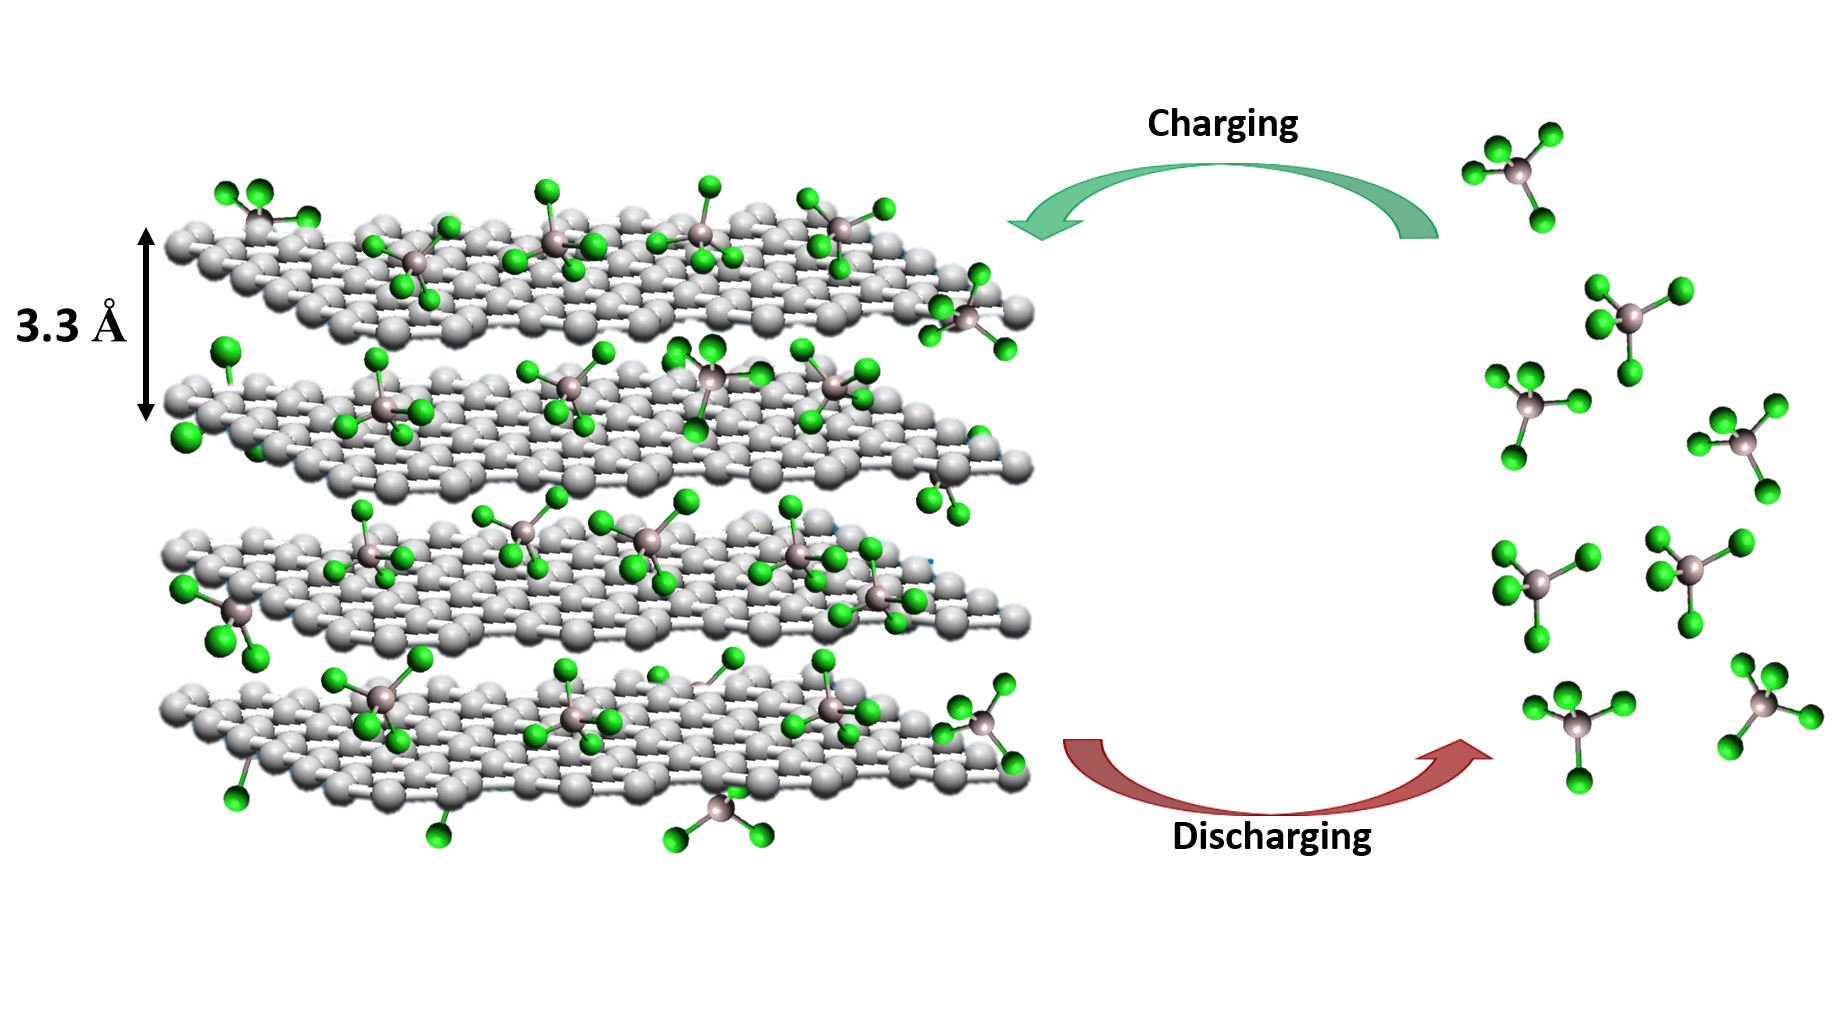
\includegraphics[width=\textwidth]{Figures/chap5fig/graphmech}
    \caption{Intercalation of \ce{AlCl4-} ions during cell charge and deintercalation during discharge in a Al/graphite cell. The interlayer distance between two graphite sheets is 3.3 \AA.}
  \label{Figures/chap5fig:graphmech}
\end{figure}

We compared four different carbon-based materials- activated carbon from human hair, activated carbon from hemp fibers, fullerenes and Super-P carbon black. Super-P carbon black is an amorphous form of carbon. It is highly conductive and is added in electrode slurries to enhance the conductivity of a cathode material. Activated carbon, also known as 'hierarchical porous carbons', derived from natural products such as rice husk, coconut shells or wood, have been previously used in batteries and super-capacitors \cite{hussain_development_2019, frackowiak_carbon_2001}. These structures contain pores of various sizes (mesopores and micropores). Mixture of \ce{C60} and \ce{C70} fullerenes was also tried as a cathode material. Fullerenes have a cage-like structure that gives them a very high surface area. Materials with high surface area adsorb ions on the surface of the material reversibly or sometimes undergo fast surface redox reactions. Based on these analogies, we tried  

\section{Results and discussion}

\begin{table}[t]
\caption{Comparing average battery metrics of all carbon cathodes} \label{table1}
{\begin{tabular}{|lcccc|}
\hline
\textbf{Active material} & {\textbf{Size}} & \textbf{Specific capacity} & \textbf{Cell efficiency} & {\textbf{Cell voltage}}\\
 & (pore size) & (mAh g$^{-1}$) & $\%$ & (V)\\
\hline
Activated carbon & 5 ${\mu}$m & 102 & 97 & 1.9 \\
from human hair & & & & \\
Fullerene extract & 8.8 \AA & 78 & 85 & 1.7 \\
Hemp fibers & 2.3 $\mu$ m & 49 & 75 & 1.8 \\
Super-P & 300 \AA & 46 & 40 & 1.5 \\
\hline  % Please only put a hline at the end of the table
\end{tabular}}
\end{table}

\begin{figure}[tbh!]
  \centering
  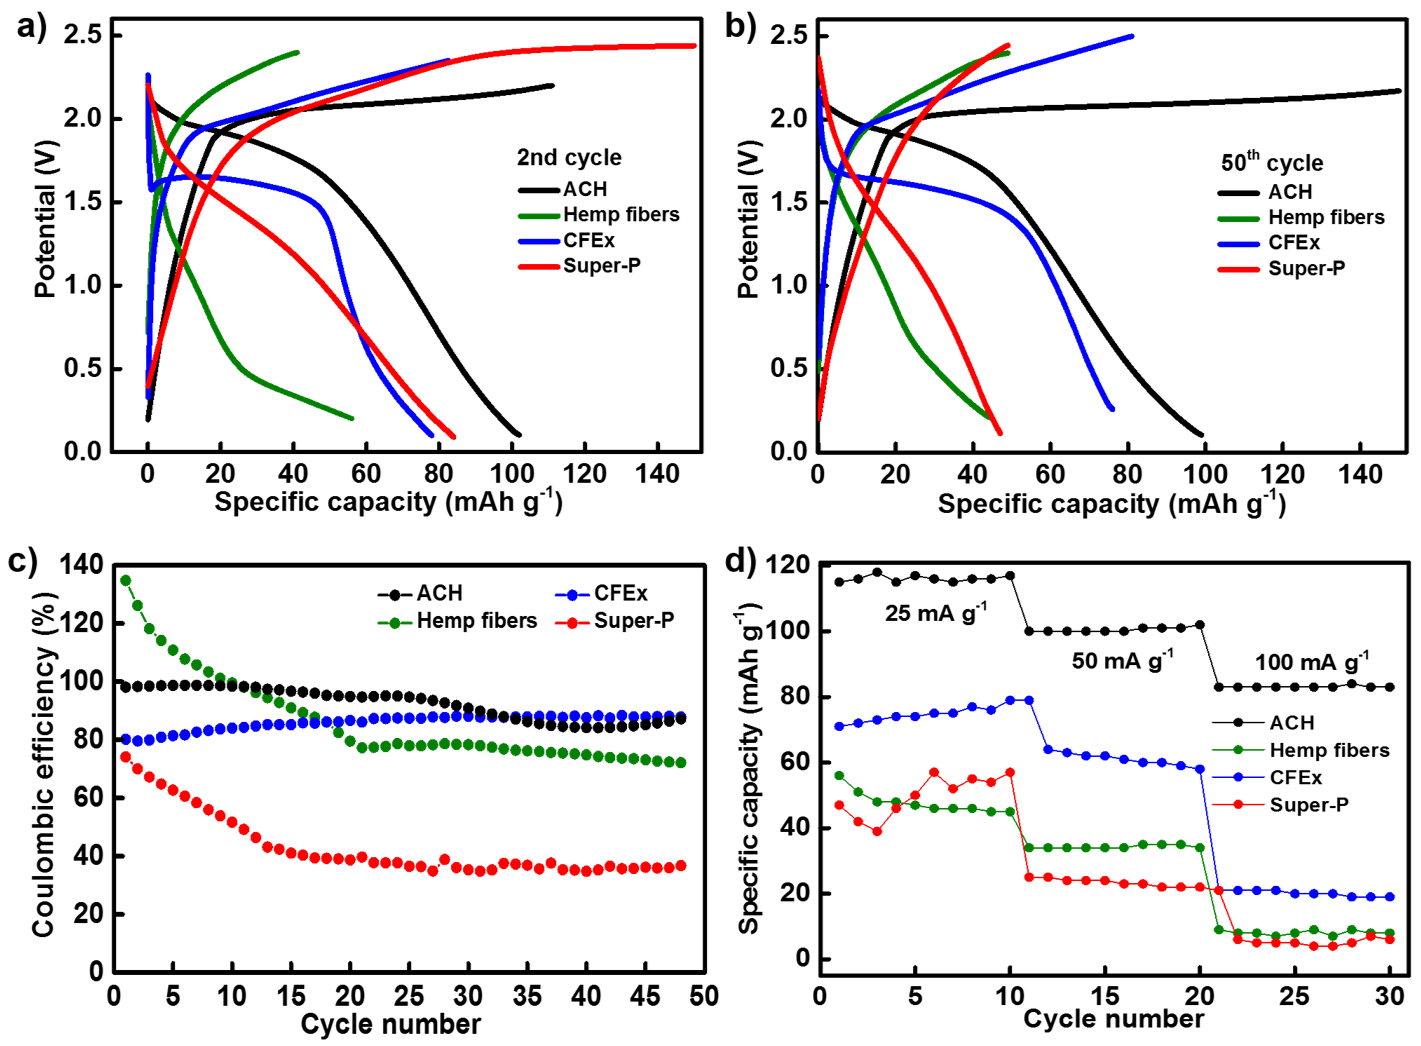
\includegraphics[width=\textwidth]{Figures/chap5fig/cdcall}
    \caption{Specific capacities in the a) 1$^{st}$ and b) 50$^{th}$ cycle of ACH, hemp fibers, CFEx and Super-P cathodes at a current rate of 50 mA g$^{-1}$. c) Cell efficiencies of cells at a current rate of 50 mAg$^{-1}$. d) Specific capacities of carbon cells at current rates of 25 mAg$^{-1}$, 50 mAg$^{-1}$ and 100 mAg$^{-1}$ in a two-electrode setup against Al$^{3+}$/Al. }
  \label{Figures/chap5fig:cdcall}
\end{figure}

ACH, hemp fibers and Super-P had an amorphous structure, however Raman spectra showed presence of a few graphitic planes. Any number of graphite-like layers would allow \ce{AlCl4-} ions to intercalate when the cell was charged. However, CFEx, a mixture of \ce{C60} and \ce{C70} fullerenes, had a crystalline lattice. Intercalation into the fullerene cage was not feasible because it needed a high amount of energy to break a C-C bond. We suggest that \ce{AlCl4-} anions seeped through the gaps present in between fullerenes without altering the molecular structure. Specific capacities of the cathodes were recorded at a constant current density of 50 mA g$^{-1}$ in Figure\ref{Figures/chap5fig:cdcall}a and b. Structural changes in the cathode before and after cycles was studied using their Raman spectra, XRD spectra and scanning electron microscopy (SEM) images.
ACH cells recorded the highest capacity at 102-mAh g$^{-1}$ and maintained it for 50 cycles. Coulombic efficiency was stable at ~95$\%$. Porous structure gave the material a high surface area that lead to an additional surface-based charge storage mechanism (observed in capacitors).Hemp fibers, due to their porous structure, observed a similar mechanism. Hemp cell showed a capacity of 56 mAh g$^{-1}$ in its first cycle, which decreased to 45 mAh g$^{-1}$ after 50 cycles. CFEx cell recorded its first discharge capacity at 79 mAh g$^{-1}$, which shifted to just 78 mAh g$^{-1}$. The cell maintained its coulombic efficiency at ~90$\%$. Specific capacity of the Super-P cell decreased considerably after repeated charge/ discharge cycles. With an initial capacity of 84 mAh g$^{-1}$, the value decreased to 47 mAh g$^{-1}$ with a low coulombic efficiency of $\sim$40$\%$. A low coulombic efficiency, also observed in hemp cells, can be attributed to degradation of cathode structure, also known as cathode pulverisation. It seems due to continuous cycling, weak bonds existing between sections of the cathode broke and agglomerated into smaller chunks of C atoms. As a result, the number of surface pores decreased, which reduced the cell's capacity (Figure \ref{Figures/chap5fig:cdcall}c). 
Human hair has two components- cuticle and cortex. One way to make carbon porous is by treating it with an activating agent. Using activating agents especially alkali hydroxides improves the porosity and increases the surface area of material \cite{liu_hair-based_2017} .
In this work, sodium hydroxide (NaOH) was used as the activating agent, which breaks the weak interactions existing between the overlapping cells in the cortex. The reaction that takes place inside the matrix after adding NaOH is:

\begin{center}
    4NaOH + C $\longrightarrow$ 4Na + 4\ce{CO2} + 2\ce{H2O} \cite{qian_human_2013}
\end{center}

NaOH was reduced to Na, these atoms in turn expanded the carbon matrix. Oxidation of carbon formed \ce{CO2}, which created pores. An increase in temperature lead to Na activation, which was later removed from the matrix via channels created by \ce{CO2}. The channels created in this process provided path for \ce {AlCl4-} to intercalate inside the pores. The activating agent:carbon ratio and the calcinating temperature played an important role in determining the size of pores. The calcinating temperature used here was 750$^{\circ}$C. A schematic of ACH synthesis has been described in Figure \ref{Figures/chap5fig:achsyn}. Dong \textit{et al.} suggested that at higher temperatures (>900$^{\circ}$C) pores start to collapse resulting in graphitic sheets \cite{dong_commercial_2019}. 
Fibers obtained from Hemp (\textit{Cannabis Sativa L.}) have been used in several commercial items including paper, textiles, clothing, biodegradable plastics, paints, and bio-fuels. They have been used as reinforcements in composite materials and are capable of replacing glass fibers. Hemp fibers have a high moisture content which can be removed after high temperature treatment\cite{hussain_development_2019}. For creating activated carbon from these fibers, potassium hydroxide (KOH) was used as the activating agent. Since the samples were obtained from Carbon Valley\textsuperscript{\textregistered}, we are unable to report the precise calcinating temperature used. Unfortunately the structural domains appeared to have been damaged after this process. This phenomena negatively impacted its charge-storing capacity.  
Fullerenes have a fused-ring structure. The nucleus-to-nucleus diameter is 7.1\AA\ and van der Waals diameter is 11 \AA in a single crystal. Presence of $\pi$-electrons on its surface makes it a good electron acceptor. However, they are zero-dimensional materials, which means they cannot provide an efficient path for electron transport or a long-range conductivity\cite{loutfy_fullerene_2002, winkler_two-component_2007}. Electrochemical reduction of \ce{C60} to \ce{C60^{-3}} is highly reversible suggesting they are capable of giving reversible capacities. However, they are weak battery cathode materials owing to their solubility in electrolytes, especially in LIBs \cite{seger_prospects_1991}. To test their solubility in \ce{AlCl3}-EMImCl ionic liquid, 100 mg of CFEx was mixed in the electrolyte and stirred for 4 hours. For comparison, we mixed hemp fibers in another vial. The vials were left to stand for 24 hours in a \ce{N2}-filled glove box. A phase separation was observed with hemp fibers but not for CFEx indicating it dissolved in the electrolyte (Figure \ref{Figures/chap5fig:cfexsol}. It has been reported in Li-S batteries that poly-sulphides produced during charge-discharge were soluble in the electrolyte. It forms an insulating layer of \ce{Li2S} on the anode, which resulted in capacity fading \cite{sun_effect_2017}. However, reversible capacities obtained after 50 cycles suggested no such molecules were formed with \ce{AlCl3}/EmImCl electrolyte. 

 \begin{figure}[tbh!]
  \centering
  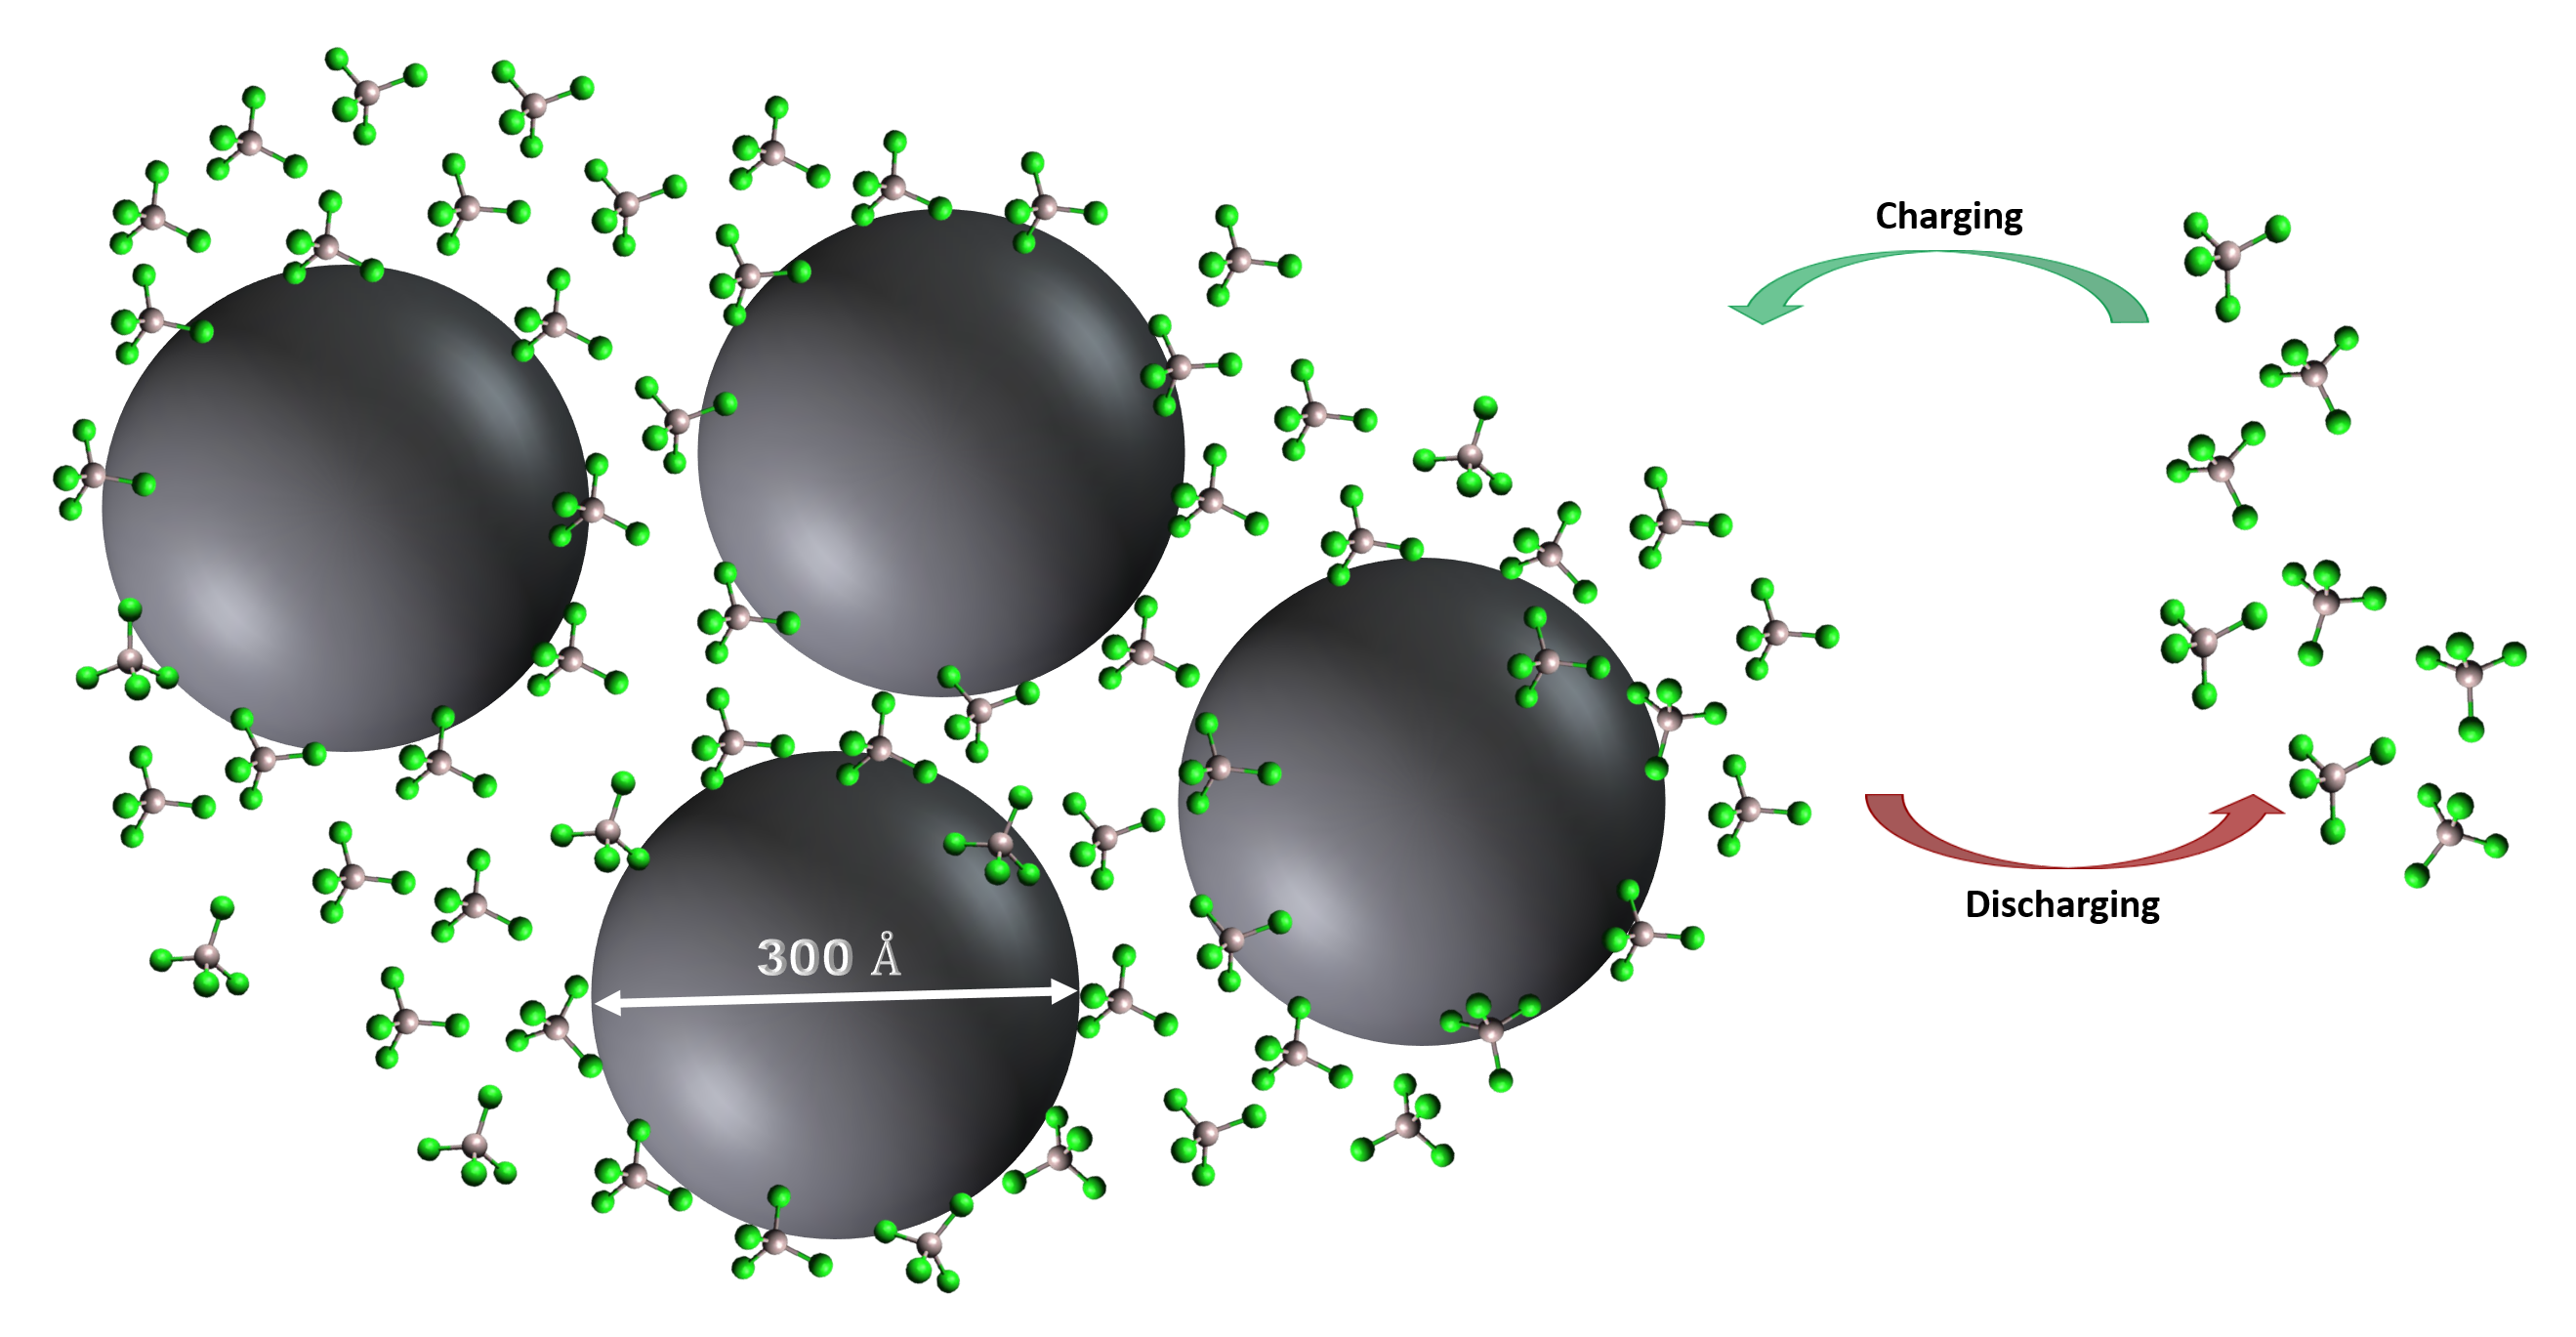
\includegraphics[width=\textwidth]{Figures/chap5fig/superpmech}
    \caption{Suggested mechanism for a \textbf{Al/Super-P} cell. Super-P has a very amorphous structure with a few graphite-like planes present in it. AlCl$_{4}^{-}$ ions intercalate into those layers and give the cell its capacity. However, cathode pulverisation results in capacity fading.}
  \label{Figures/chap5figs:superPmech}
\end{figure}

Pore size for Super-P ranges from ~30-50 nm \cite{younesi_analysis_2015}. It has the least graphitic structure when compared to ACH and hemp fibers. Loosely held structures, which disintegrated rapidly after every cycle resulted in reduced capacity and low coulombic efficiency values.

 \begin{figure}[tbh!]
  \centering
  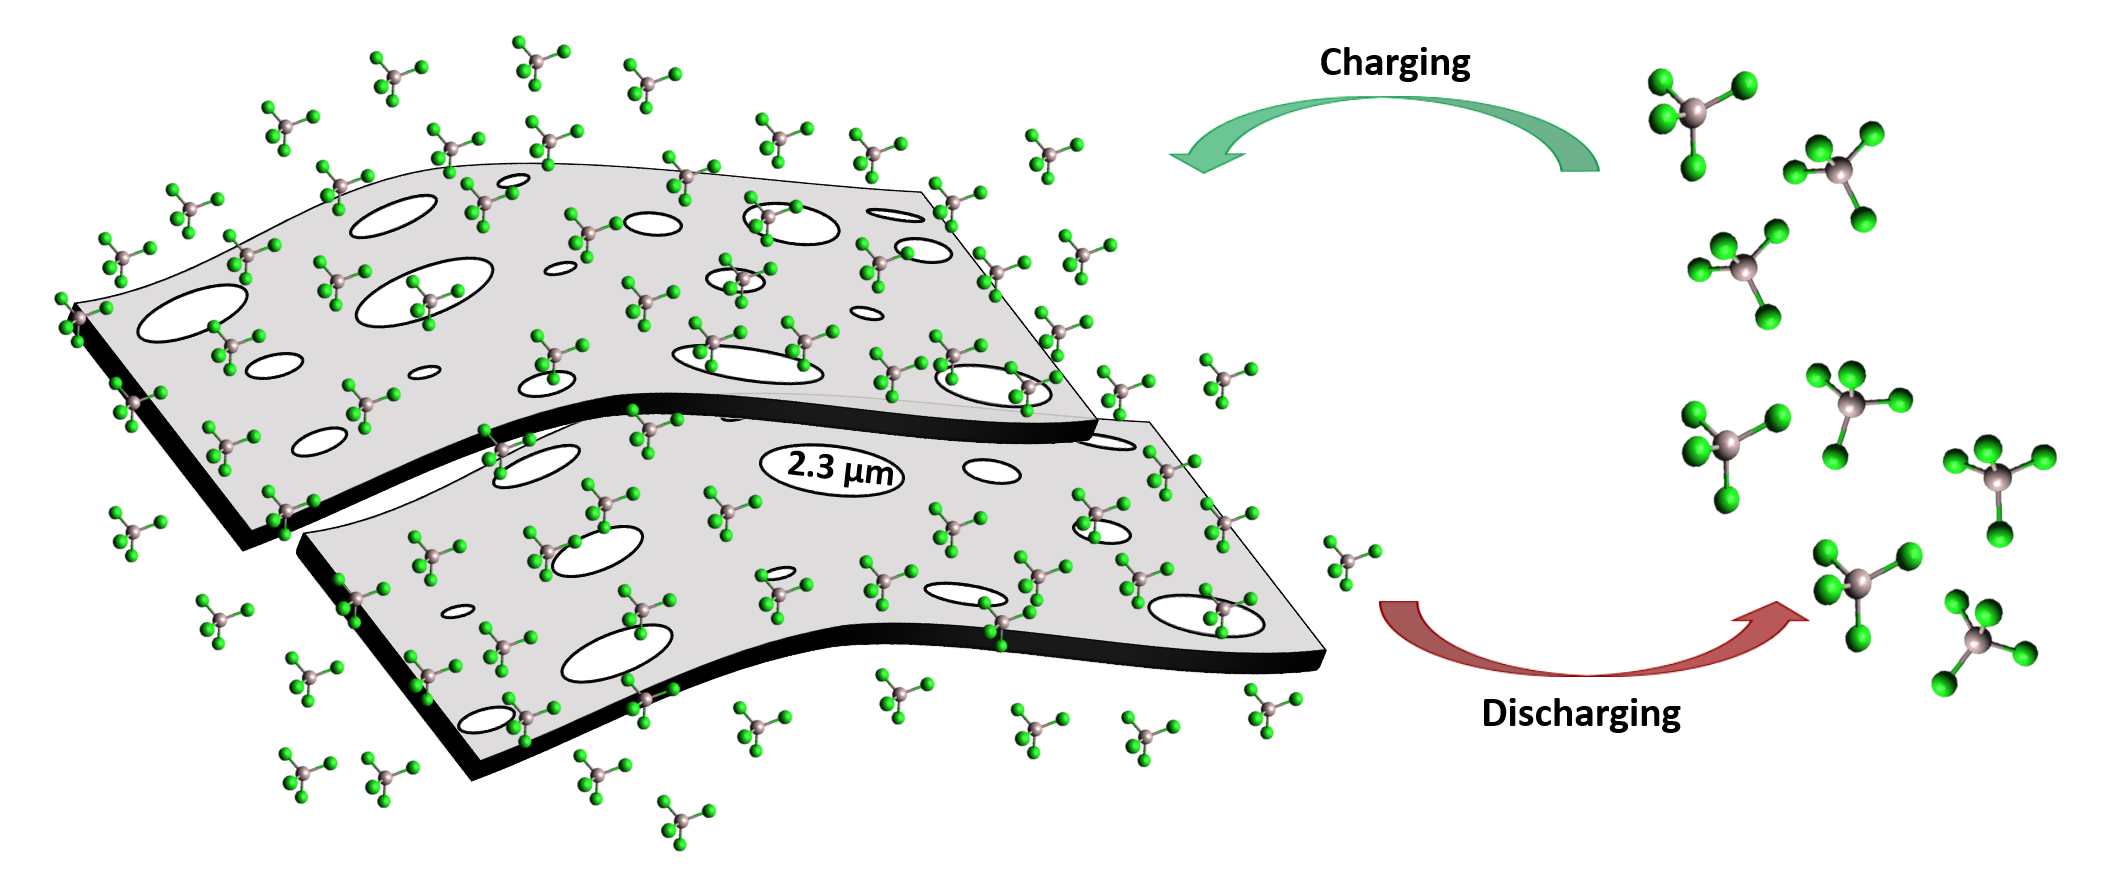
\includegraphics[width=\textwidth]{Figures/chap5fig/hempmech}
    \caption{Suggested mechanism for a \textbf{Al/hemp} cell. The fibers have a large pore size (2.0-2.5 $\mu$m) which allow the \ce{AlCl4-} to get absorbed on the cathode surface but agglomeration of carbon atoms after a few cycles reduces the active sites available for charge storage, which reduces cell's capacity after every cycle.}
  \label{Figures/chap5fig:hempmech}
\end{figure}

 \begin{figure}[tbh!]
  \centering
  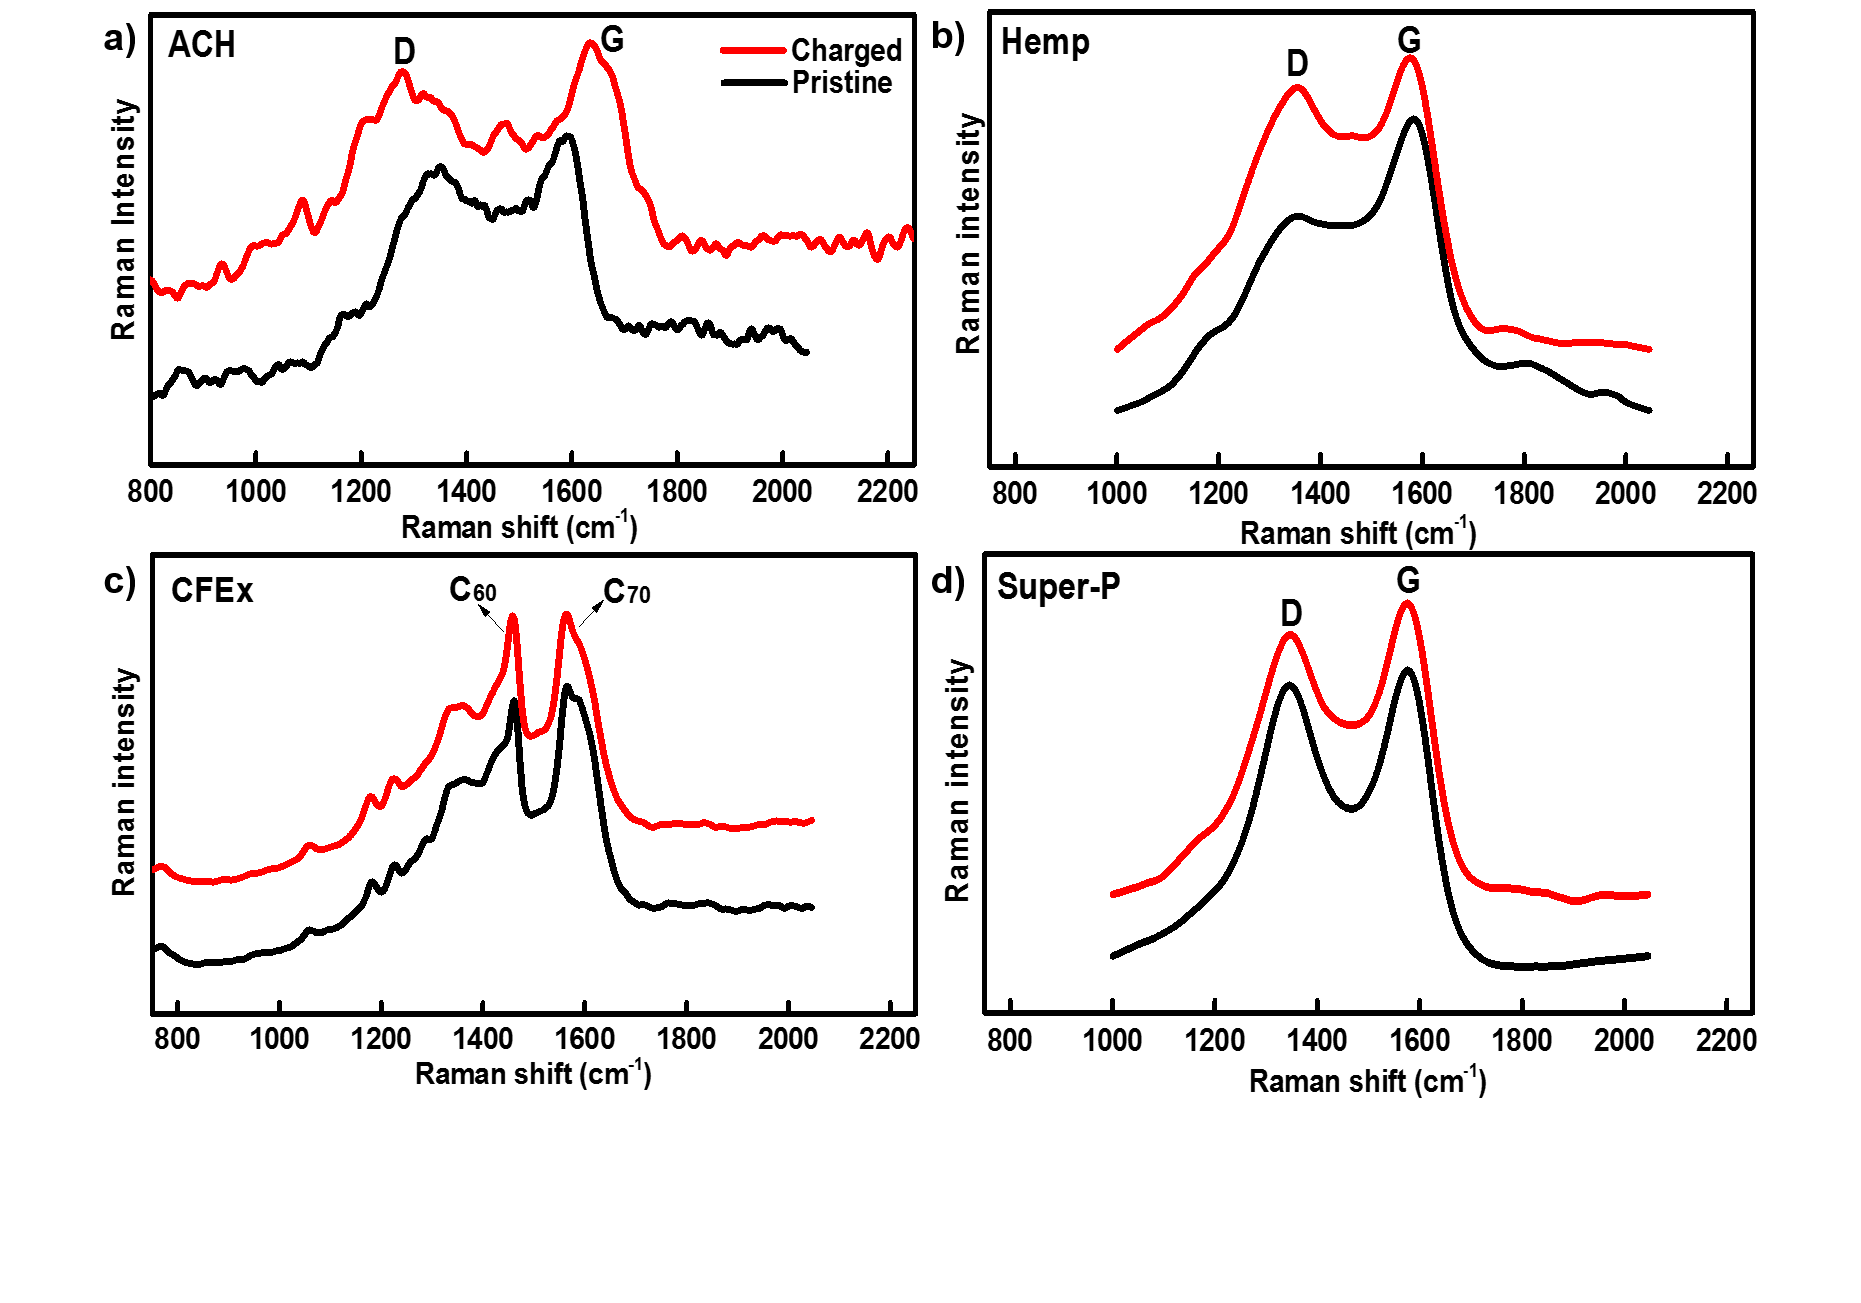
\includegraphics[width=\textwidth]{Figures/chap5fig/Raman}
    \caption{Raman spectra of pristine (in black) and charged (in red) a) CFEx , b) hemp fibers, c) ACH and d) Super-P cathodes indicating presence of both D and G-bands.}
  \label{Figures/chap5fig:Raman}
\end{figure}

Since it has been previously established that intercalation of \ce{AlCl4-} takes place in carbon materials during cell charge, we focused our analysis on the charged electrodes. Figure \ref{Figures/chap5fig:Raman} illustrates Raman spectra of the tested cathodes. Pristine ACH, hemp fibers and Super-P had a significant D-band indicating a distorted lattice. Increased intensity of D band can be seen in charged electrodes at ~1300 cm$^{-1}$ (ACH), 1329.7 cm$^{-1}$ (hemp fibers), and 1352.0 cm$^{-1}$ (Super-P) indicating an increase in the lattice defects and deformities. Hemp fibers and ACH observed an increased FWHM (full width at half maximum) of both D and G bands indicating a loss in symmetry. Intercalation of ions or surface adsorption of anions onto the porous carbon cathode, would alter the ordered structure on the surface. We suggest capacitive intercalation mechanism as well as a redox pseudocapacitance where \ce{AlCl4-} ions electrochemically adsorb onto the surface \cite{brezesinski_ordered_2010}. 
The main feature in a fullerene Raman spectrum was a sharp line observed at 1460 cm$^{-1}$, which is known as the 'pentagonal pinch mode'. \ce{C60} is composed of \ce{sp2} bonded carbon atoms. Sharpness of the band indicates a uniform nature of the bonds. However, the spectrum of \ce{C70} has multiple bands. Reduction in its molecular symmetry increases the number of active Raman bands \cite{kimbrell_analysis_2014}. Pristine CFEx electrode observed characteristic peaks of both \ce{C60} and \ce{C70} at 1459.3 cm$^{-1}$ and 1564 cm$^{-1}$ respectively in Figure \ref{Figures/chap5fig:Raman}c. An interesting observation was that pristine and charged CFEx electrodes had a similar-looking spectra after cycling. Since Raman spectroscopy is sensitive to very minute differences in molecular morphology, the results suggested that the structure remained intact. Another interesting observation was made in charged ACH electrode (Figure \ref{Figures/chap5fig:Raman}a). A new peak appeared at 1466 cm$^{-1}$. A similar band splitting was observed by Wang \textit{et al} \cite{wang_kish_2017} while charging natural graphite and \ce{AlCl4-} ions intercalated into the cathode layers. This peak appeared due to vibration of carbon atoms in a plane adjacent to intercalant layer planes. We observed no such effect was observed for any other cathode. Since the Al/ACH cell maintained a highly reversible capacity of 102 mAhg$^{-1}$ after 50 cycles, we assume ACH underwent a similar mechanism, where \ce{AlCl4-} ions intercalate into the cathode during charge. ACH has a high surface area and an inter-connected mesoporosity. The layered domains present in it enable insertion of \ce{AlCl4-}, while a few anions get electrochemically adsorbed onto the surface through a charge-transfer process resulting in a redox pseudo-capacitance. All these processes seem to take place at the same time without changing the reaction kinetics. Additionally, presence of both an amorphous and crystalline structure in this material increases the charge-storage capacity of the material \cite{brezesinski_ordered_2010}. This might be the reason why ACH shows a remarkable reversibility. Schematic of a possible mechanism is shown in Figure \ref{Figures/chap5fig:achmech}. Hemp fibers and Super-P had lattice deformities to begin with, which were enhanced after the cell underwent the preliminary galvanostatic cycles. This decreased capacity after every cycle. 

\begin{figure}[tbh!]
  \centering
  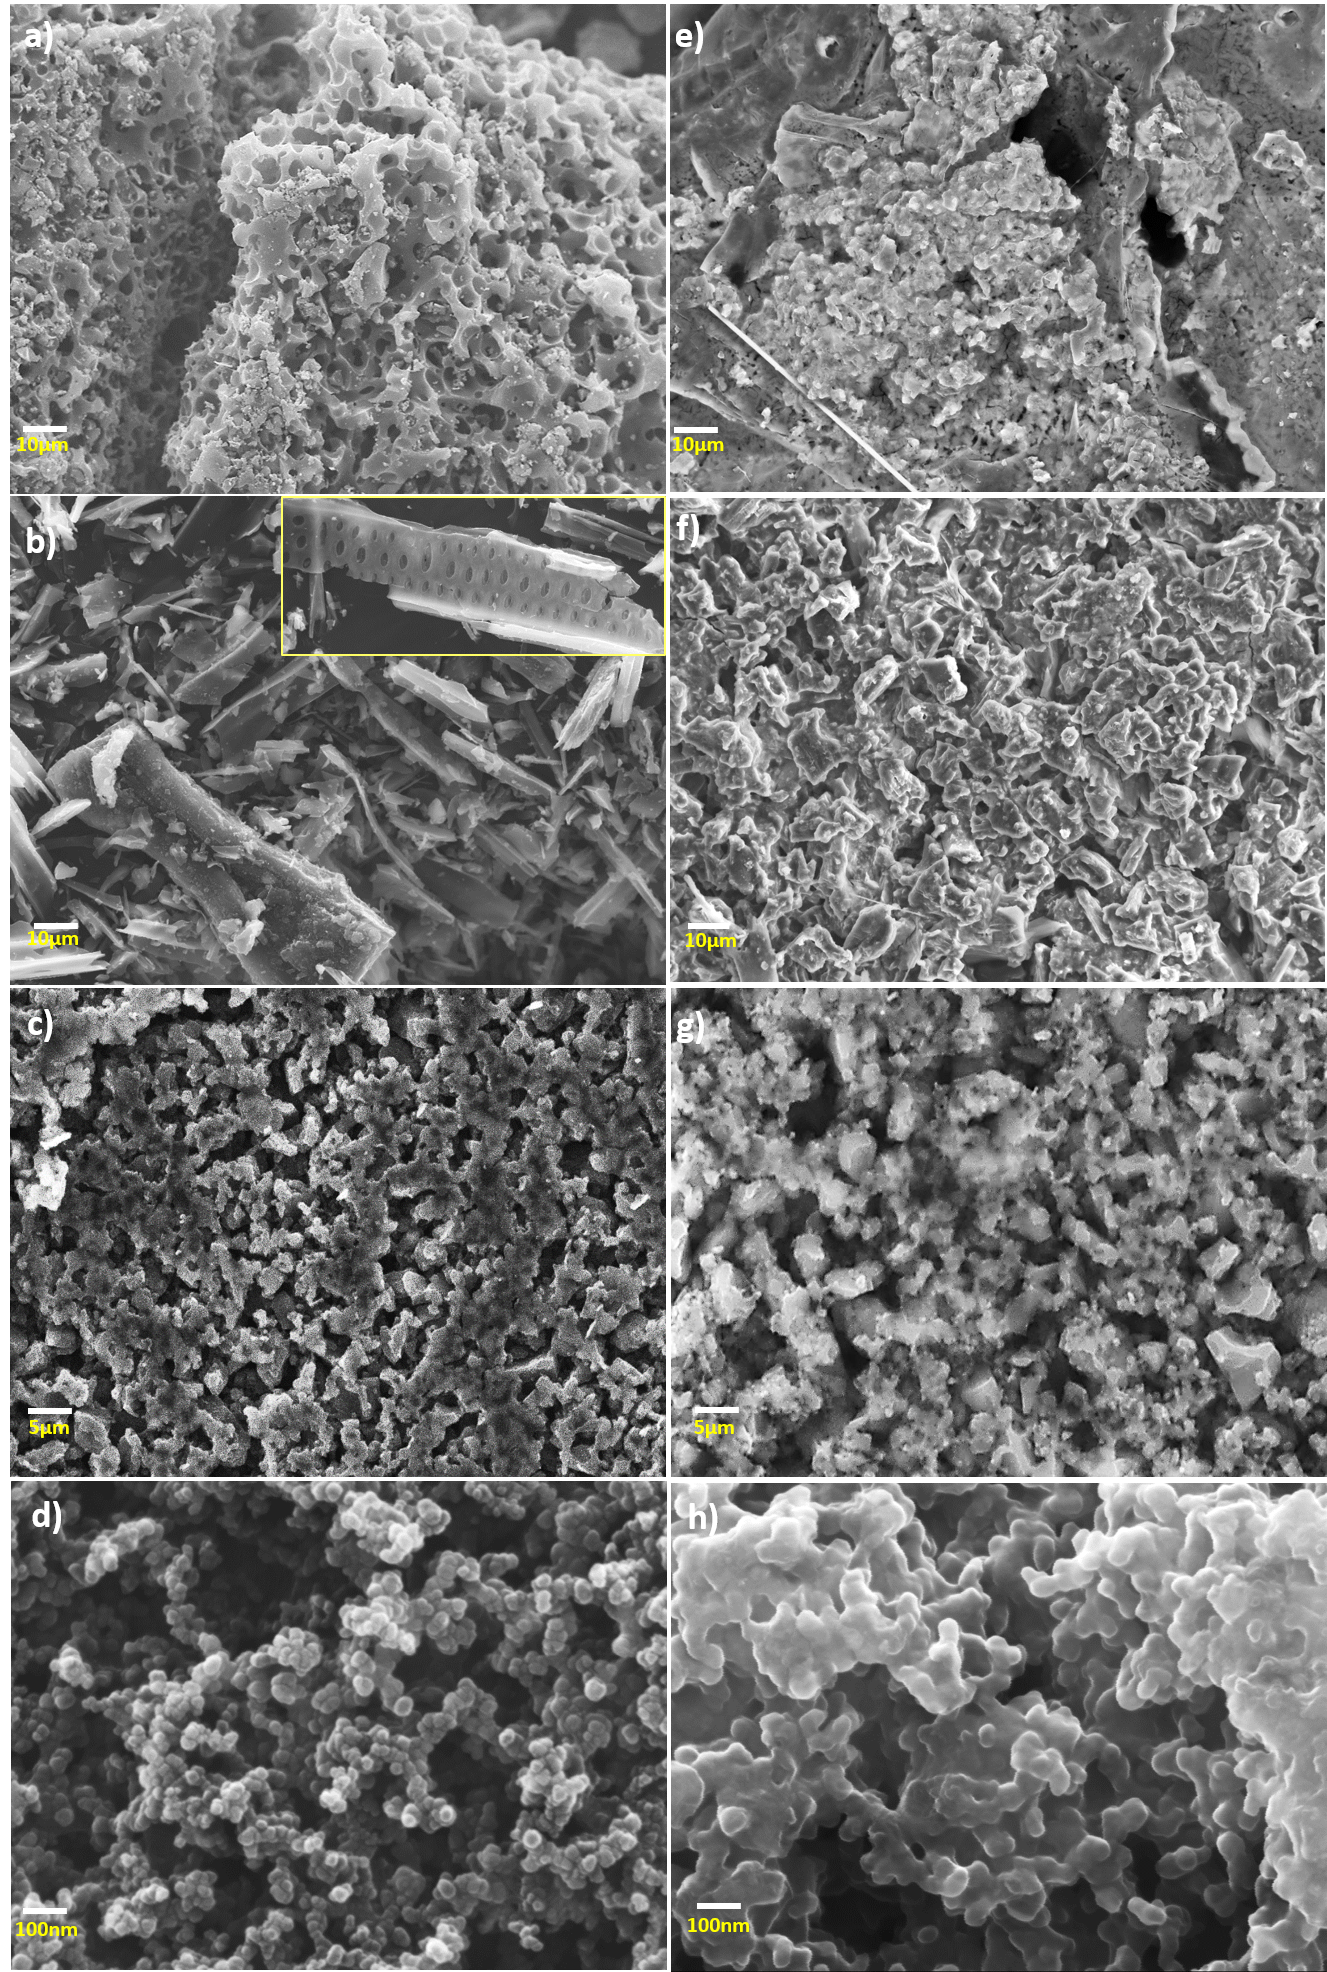
\includegraphics[width=0.6\textwidth]{Figures/chap5fig/SEM}
    \caption{Scanning electron microscopy images comparing pristine a) ACH, b) hemp fibers, c) CFEx and d) Super-P; and charged e)ACH, f) hemp fibers, g) CFEx and h) Super-P electrodes. Hemp fibers and Super-P undergo prominent changes after charge/discharge cycles (visible agglomeration of carbon atoms).}
  \label{Figures/chap5fig:SEM}
\end{figure}

Above results seem to be in good agreement with SEM images in Figure 9, where we compared pristine (Figure \ref{Figures/chap5fig:SEM}a, b, c and d) and charged electrodes (\ref{Figures/chap5fig:SEM}e,f,g and h). ACH and hemp fibres have a porous structure (Figure \ref{Figures/chap5fig:SEM}a and 9b), which looked visibly degraded after cycles (Figure \ref{Figures/chap5fig:SEM}e and f). Agglomeration of carbon atoms increases the edge defects in a material. This explains the high intensity of D-bands of these cathodes, Figure \ref{Figures/chap5fig:Raman}. Surface morphology of CFEx (Figure \ref{Figures/chap5fig:SEM}c did not change a lot after charge (Figure \ref{Figures/chap5fig:SEM}g), similar to our observations in its Raman spectra. 
\begin{figure}[tbh!]
  \centering
  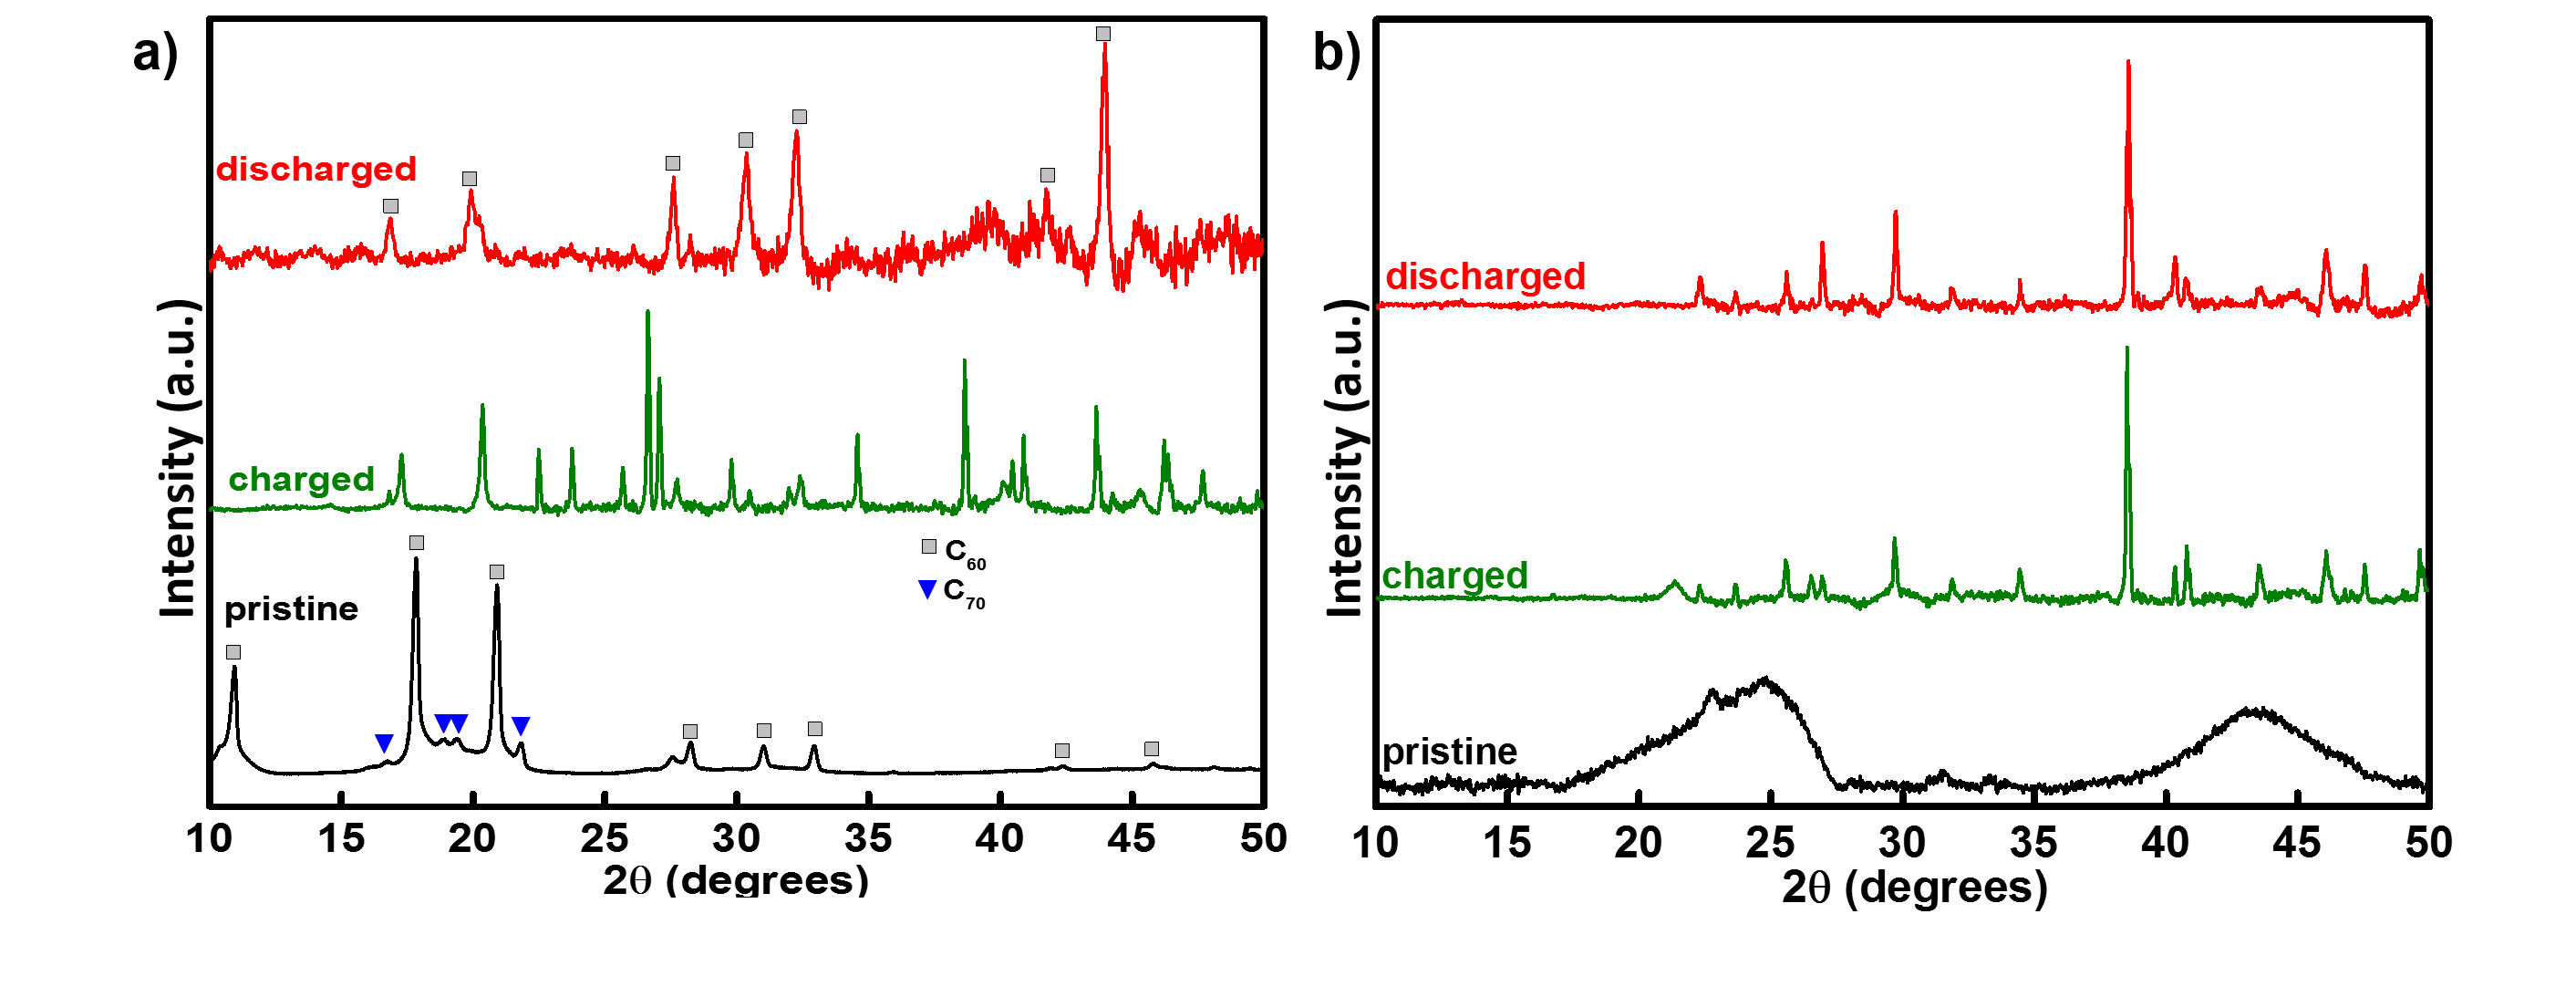
\includegraphics[width=\textwidth]{Figures/chap5fig/xrd}
    \caption{XRD spectra comparing a pristine (black), charged (green) and discharged (red) a) CFEx and b)ACH cathode to study changes in their lattice after 50 galvanostatic cycles in a two-electrode setup against \ce{Al$^{3+}$/Al} with characteristic peaks marked for \ce{C60} (in grey) and \ce{C70} (in blue).}
  \label{Figures/chap5fig:xrd}
\end{figure}

To confirm the reversible electrochemical processes taking place in CFEx and ACH, we examined their XRD spectra (pristine, charged and discharged) in Figure \ref{Figures/chap5fig:xrd}a and b respectively. Pristine cathode recorded the characteristic peaks of both \ce{C60} and \ce{C70}, which reappeared after discharge suggesting a reversible process. However, charged electrode observed new diffraction peaks which can be attributed to lattice deformities taking place at the electrode/electrolyte interface. We calculated the unit cell lattice parameters for both pristine and charged cathode for a \ce{C60} molecule. The unit cell had a tetragonal crystal system with space group of P42/mmc and a space group number 131 (ICDD: 04-013-1339 for \ce{C60}). Lattice parameter 'a' and 'b' for the charged electrode changed from 9.06 \AA to 9.57 \AA . Lattice parameter 'c' changed from 15.03 \AA to 15.65 \AA, in Figure \ref{Figures/chap5fig:cfexcrys}a and b. Lattice parameters for discharged cathode were closer to pristine values. The changes in the fullerene structure suggested a reversible intercalation process taking place, where the unit cells shifted from their original location during charge and returned back after discharge. A possible site for \ce{AlCl4-} intercalation is depicted in Figure \ref{Figures/chap5fig:cfexcrys}c. XRD spectra for ACH electrodes was inconclusive (Figure \ref{Figures/chap5fig:xrd}b). Pristine cathode observed very broad peaks suggesting the extreme amorphous nature of the material. However, the material seemed to have a more ordered structure after the galvanostatic cycles. It seems that surface-based charge-storage was more dominant than the intercalation process. This is why presence of crystallinity in the active material does not limit the surface-based charge storage and therefore, the capacity remains same \cite{kim_synthesis_2006, jow_factors_2018}. 

 \begin{figure}[tbh!]
  \centering
  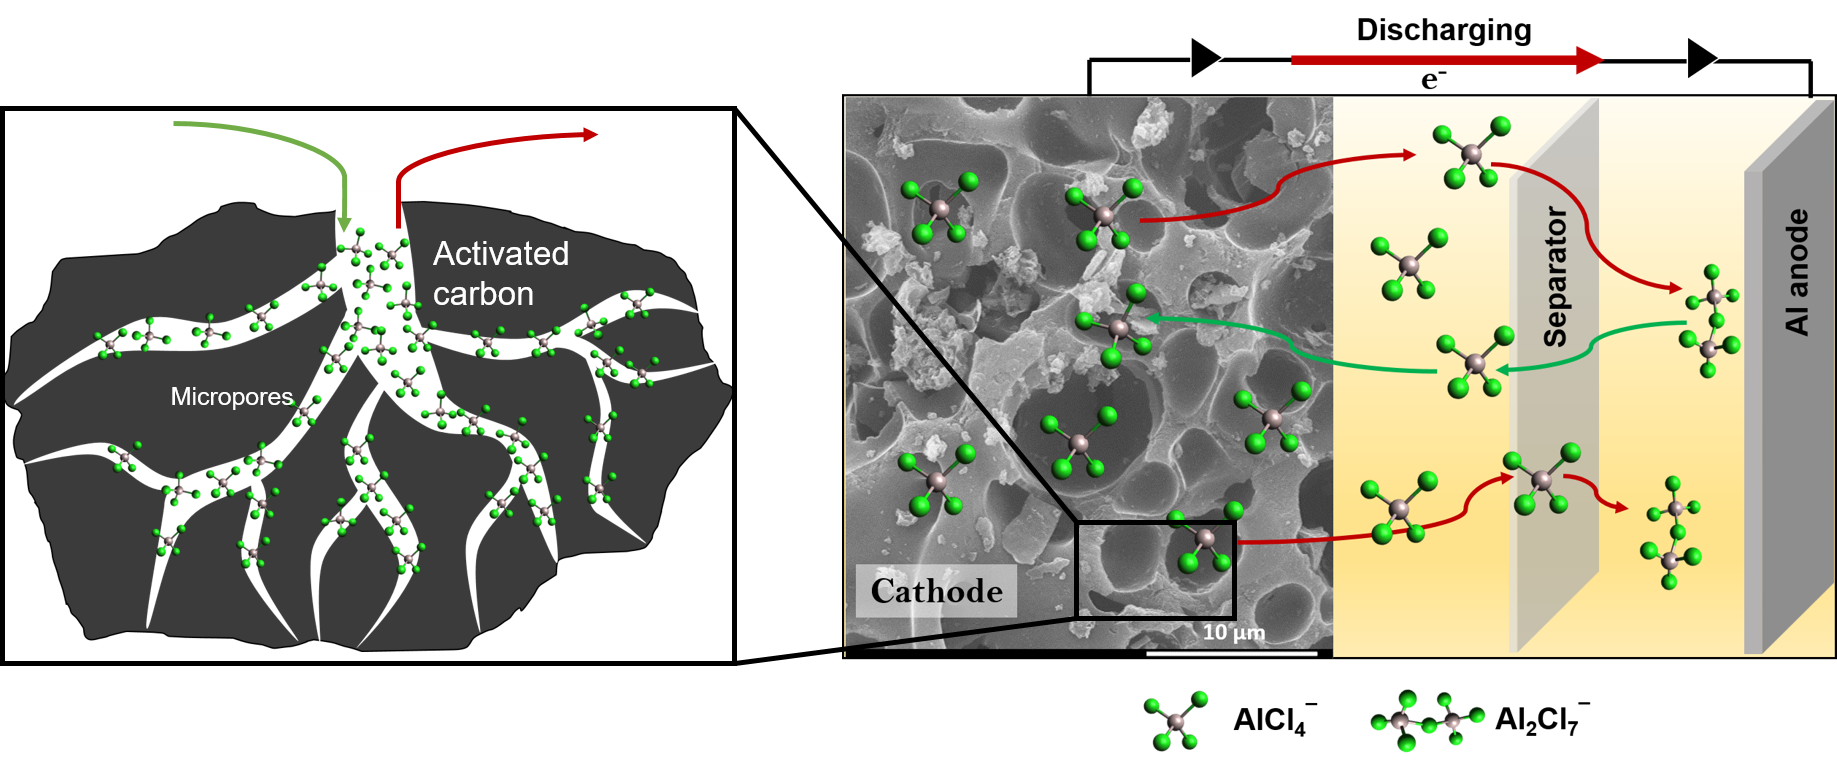
\includegraphics[width=\textwidth]{Figures/chap5fig/achmech}
    \caption{Suggested mechanism for a \textbf{Al/ACH} cell. ACH has a porous structure which allows \ce{AlCl4-} ions to get absorbed as well as reversibly intercalate into the graphitic planes, giving additional capacity to the cell.}
  \label{Figures/chap5fig:achmech}
\end{figure}

\begin{figure}[tbh!]
  \centering
  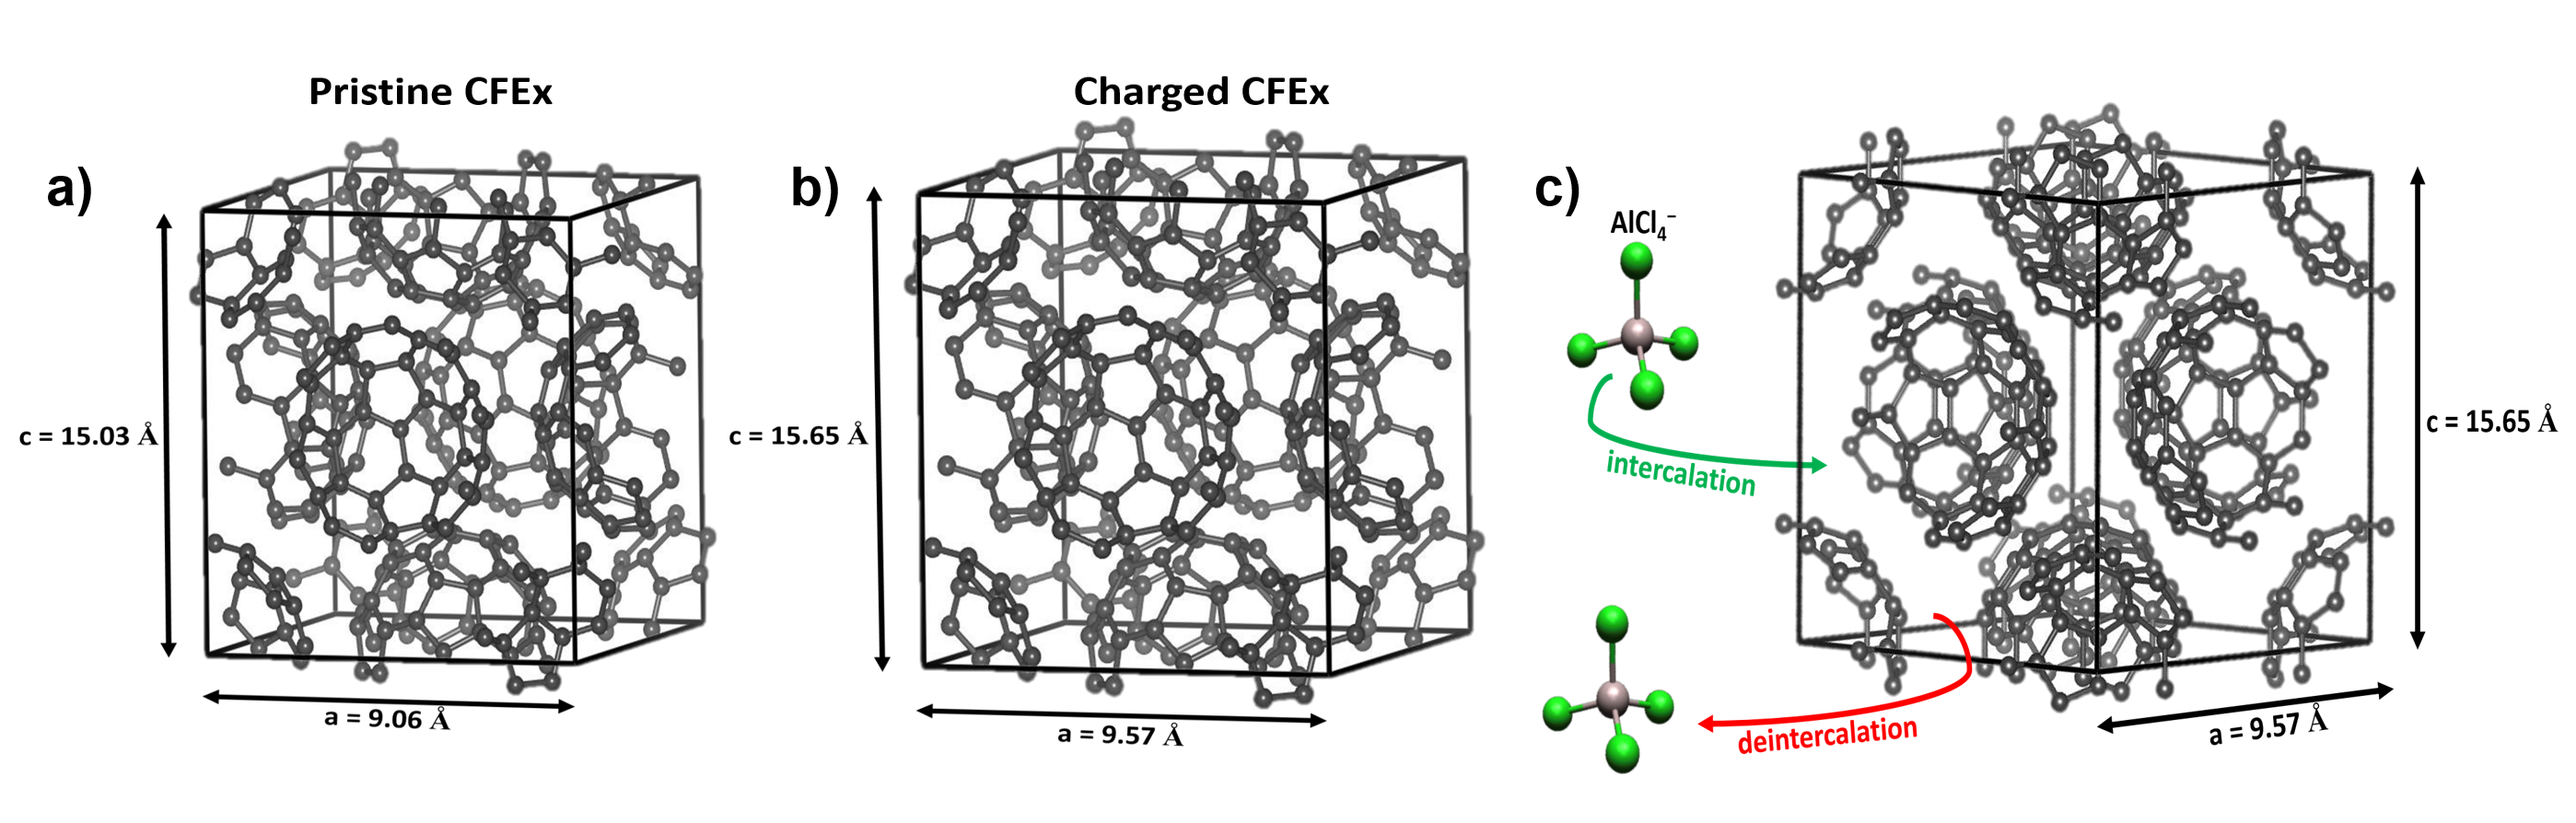
\includegraphics[width=\textwidth]{Figures/chap5fig/cfexcrys}
    \caption{Changes in the lattice parameters of a \ce{C60} unit cell. a) Pristine \ce{C60}unit cell, b) charged \ce{C60}unit cell with increased parameters suggesting a uniform shift in the lattice after charge/discharge. c) Expected intercalation sites of \ce{AlCl4-} ions in the unit cell.}
  \label{Figures/chap5fig:cfexcrys}
\end{figure}

%Charged Super-P and hemp fiber electrodes underwent degradation and appeared clumped together resulting in capacity decay. This was visible from their electrochemical results where a rapid decrease in capacity and cell efficiency was noted. 
%XPS analysis results... C 1s 
\begin{figure}[tbh!]
  \centering
  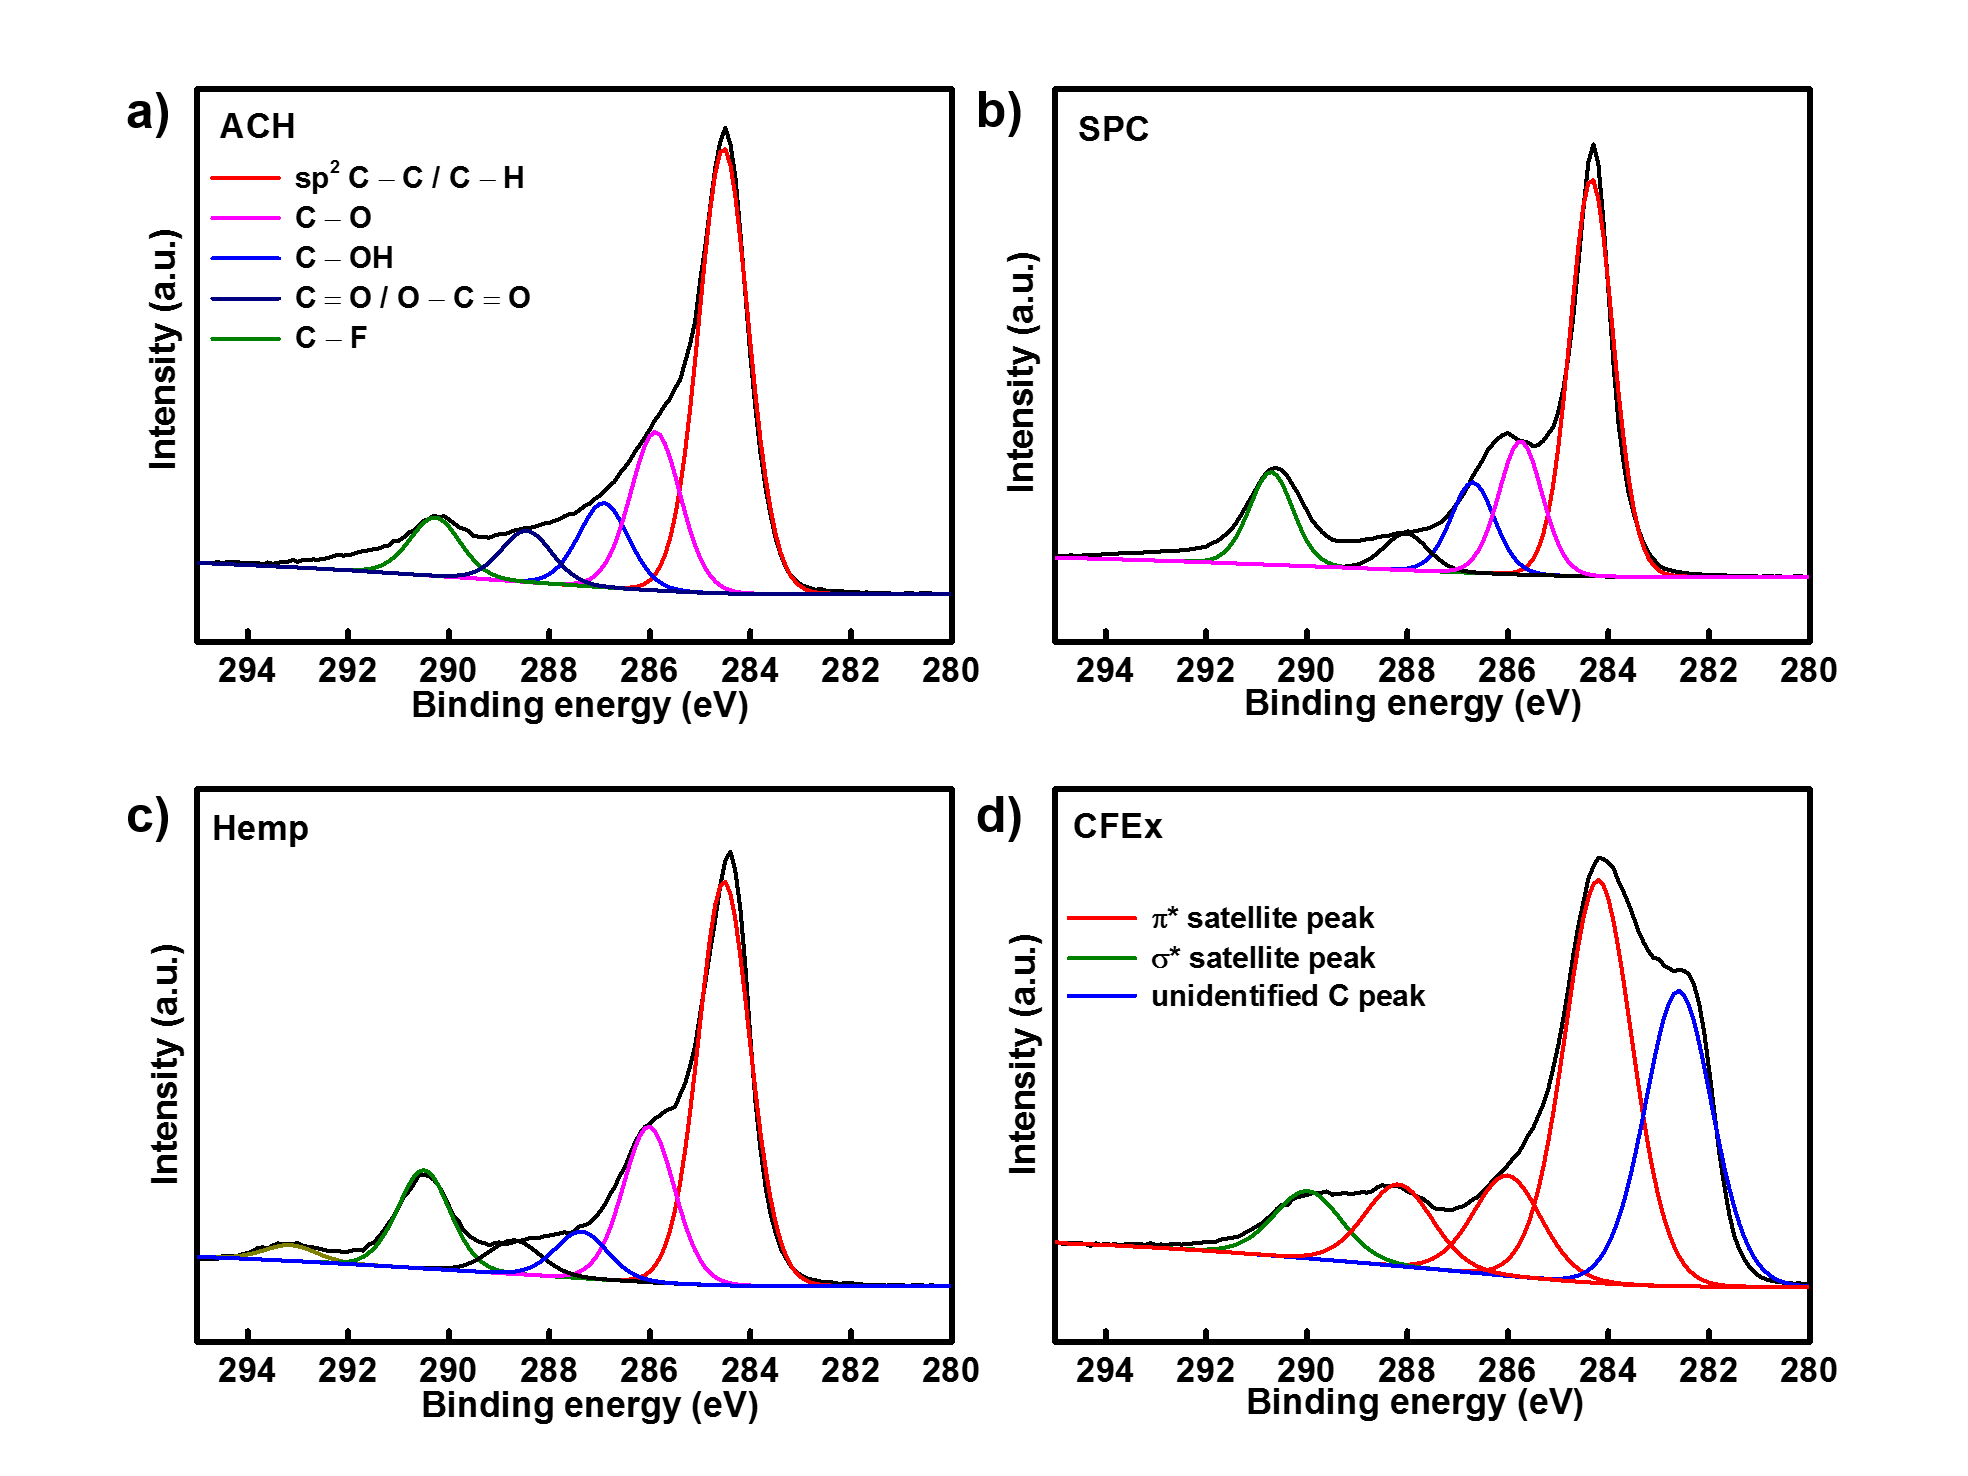
\includegraphics[width=\textwidth]{Figures/chap5fig/xpsc}
    \caption{Carbon 1s XPS spectra of pristine a) ACH, b) Super-P, c) hemp fibers and d) CFEx cathodes.While ACH, Super-P and hemp fibers observe carbonyl functional groups, CFEx cathodes have symmetrical looking $\pi$* and $\sigma$* satellite peaks.}
  \label{Figures/chap5fig:xpsc}
\end{figure}

We performed X-ray photoelectron spectroscopy on our cathodes to understand the kinds of reactions the cathodes could take part in. We observed ACH, hemp fibers and Super-P had similar looking peaks for carbon 1s orbital, Figure \ref{Figures/chap5fig:xpsc}. Peaks for sp$^2$ C-C/ C-H, C-O/ C-OH, O-C=O/ C=O and C-F bonds (formed between PVDF and the active material) appeared for ACH, hemp fibers and Super-P cathodes. To understand the presence of these bonds,we looked into the composition of these active materials. Hair is mainly composed of a protein called keratin displayed in Figure \ref{Figures/chap5fig:keratin}. Keratin constitutes of various C-H, C=O, C-OH and C-NH$_2$ bonds with their respective binding energies as observed in Figure \ref{Figures/chap5fig:xpsc}a. Sulphur is an essential part of this protein, a C-S bond can be observed at 286.94 eV (blue peak). 

\begin{table}
\caption{XPS data sheet for the tested cathodes with \textbf{Carbon 1s} peaks pointing C-H/ C-C, C-O/ C-OH, C=O/ O-C=O and C-F bonds, \textbf{Nitrogen 1s} peaks for pyrrolic and pyridnic N nods and \textbf{Oxygen 1s} peaks for aliphatic C-O and aromatic C=O peaks.} \label{table2}
\resizebox{\textwidth}{!}
{\begin{tabular}{|cccccccc|}
\hline
\textbf{Active} & \textbf{C-H/} & \textbf{C-O/} & \textbf{C=O/} & \textbf{C-F} & \textbf{Pyrrolic N/} & \textbf{aliphatic C-O} & \textbf{aromatic C=O}\\
\textbf{material} & \textbf{C-C} & \textbf{C-OH} & \textbf{O-C=O} & & \textbf{Pyridinic N} & & \\
\hline\\
ACH & 284.5 eV & 285.8 eV & 288.4 eV & 290.2 eV & 400.2 eV/ & 533.0 eV & 531.2 eV\\
& & & & & 398.3 eV & & \\
CFEx & 284.2 eV & 286.0 eV & 288.2 eV & 290.0 eV & 399.3 eV & 531.3 eV & 530.2 eV\\
Hemp fibers & 284.5 eV & 286.0 eV & 288.7 eV & 290.5 eV & 400.3 eV & 532.9 eV & 531.4 eV\\
Super-P & 284.3 eV & 286.7 eV & 288.0 eV & 290.7 eV & 400.2 eV & 532.8 eV & ---\\
\hline
\end{tabular}}
\end{table}

The oxygen-containing carbonyl and ester groups improve the wettability of cathode materials. It increases the availability of active surface area for the ions from the electrolyte to interact with the carbon matrix \cite{younesi_analysis_2015}. This enhances the pseudocapacitance of the cell since most of the capacity comes from a surface-based charge storage mechanism. Pristine hemp fibers and Super-P observed peaks for both sp$^2$ bonded carbon atoms and carbon-oxygen bonds \cite{hussain_development_2019}. Hemp fibers are composed of proteins called lignin (Figure \ref{Figures/chap5fig:lignin}), edestin and albumin which constitutes of arginine (Figure \ref{Figures/chap5fig:arginine}) and glutamic acid (Figure \ref{Figures/chap5fig:gluacid}).  

Carbon 1s spectrum of Super-P consists of contribution from O–C–O and/or C=O bonds and a strong \ce{CH2}/\ce{CF2} bond. The material is produced from partial oxidation of petrochemical precursors exhibiting a large specific surface area and a very high electrical conductivity \cite{gnanamuthu_electrochemical_2011}. Carbon black consists of nearly spherical primary particles, which are fused together in form of aggregates. A perfect graphite surface containing only carbon atoms, without heteroatoms like oxygen and sulfur would give a very well-ordered structure. Therefore, presence of carbonyl groups created defects resulting in a less graphitic and more amorphous structure\cite{hao_carbonaceous_2013}. 
Carbon spectra for CFEx electrode was uniquely different with highly symmetrical peaks. The presence of $\pi$ electrons on fullerene's surface renders multiple $\pi$ satellite peaks. These peaks are characteristic signs of a \ce{C60} molecule \cite{skryleva_xps_2016}. The symmetrical peaks in the low energy range, 284–289 eV, have C 1s excitation to final states of $\pi$* character (in red), while the higher energy peaks appear due to C 1s excitation to final states of $\sigma$* character (in green) \cite{erbahar_spectromicroscopy_2016, poirier_carbon_1993}. %Existence of several peaks in the $\pi$ satellite of a C$_6_0$ molecule is caused by the angular quantisation of orbitals around the centre of the spherical molecule. 
%XPS analysis results... O 1s

\begin{figure}[tbh!]
  \centering
  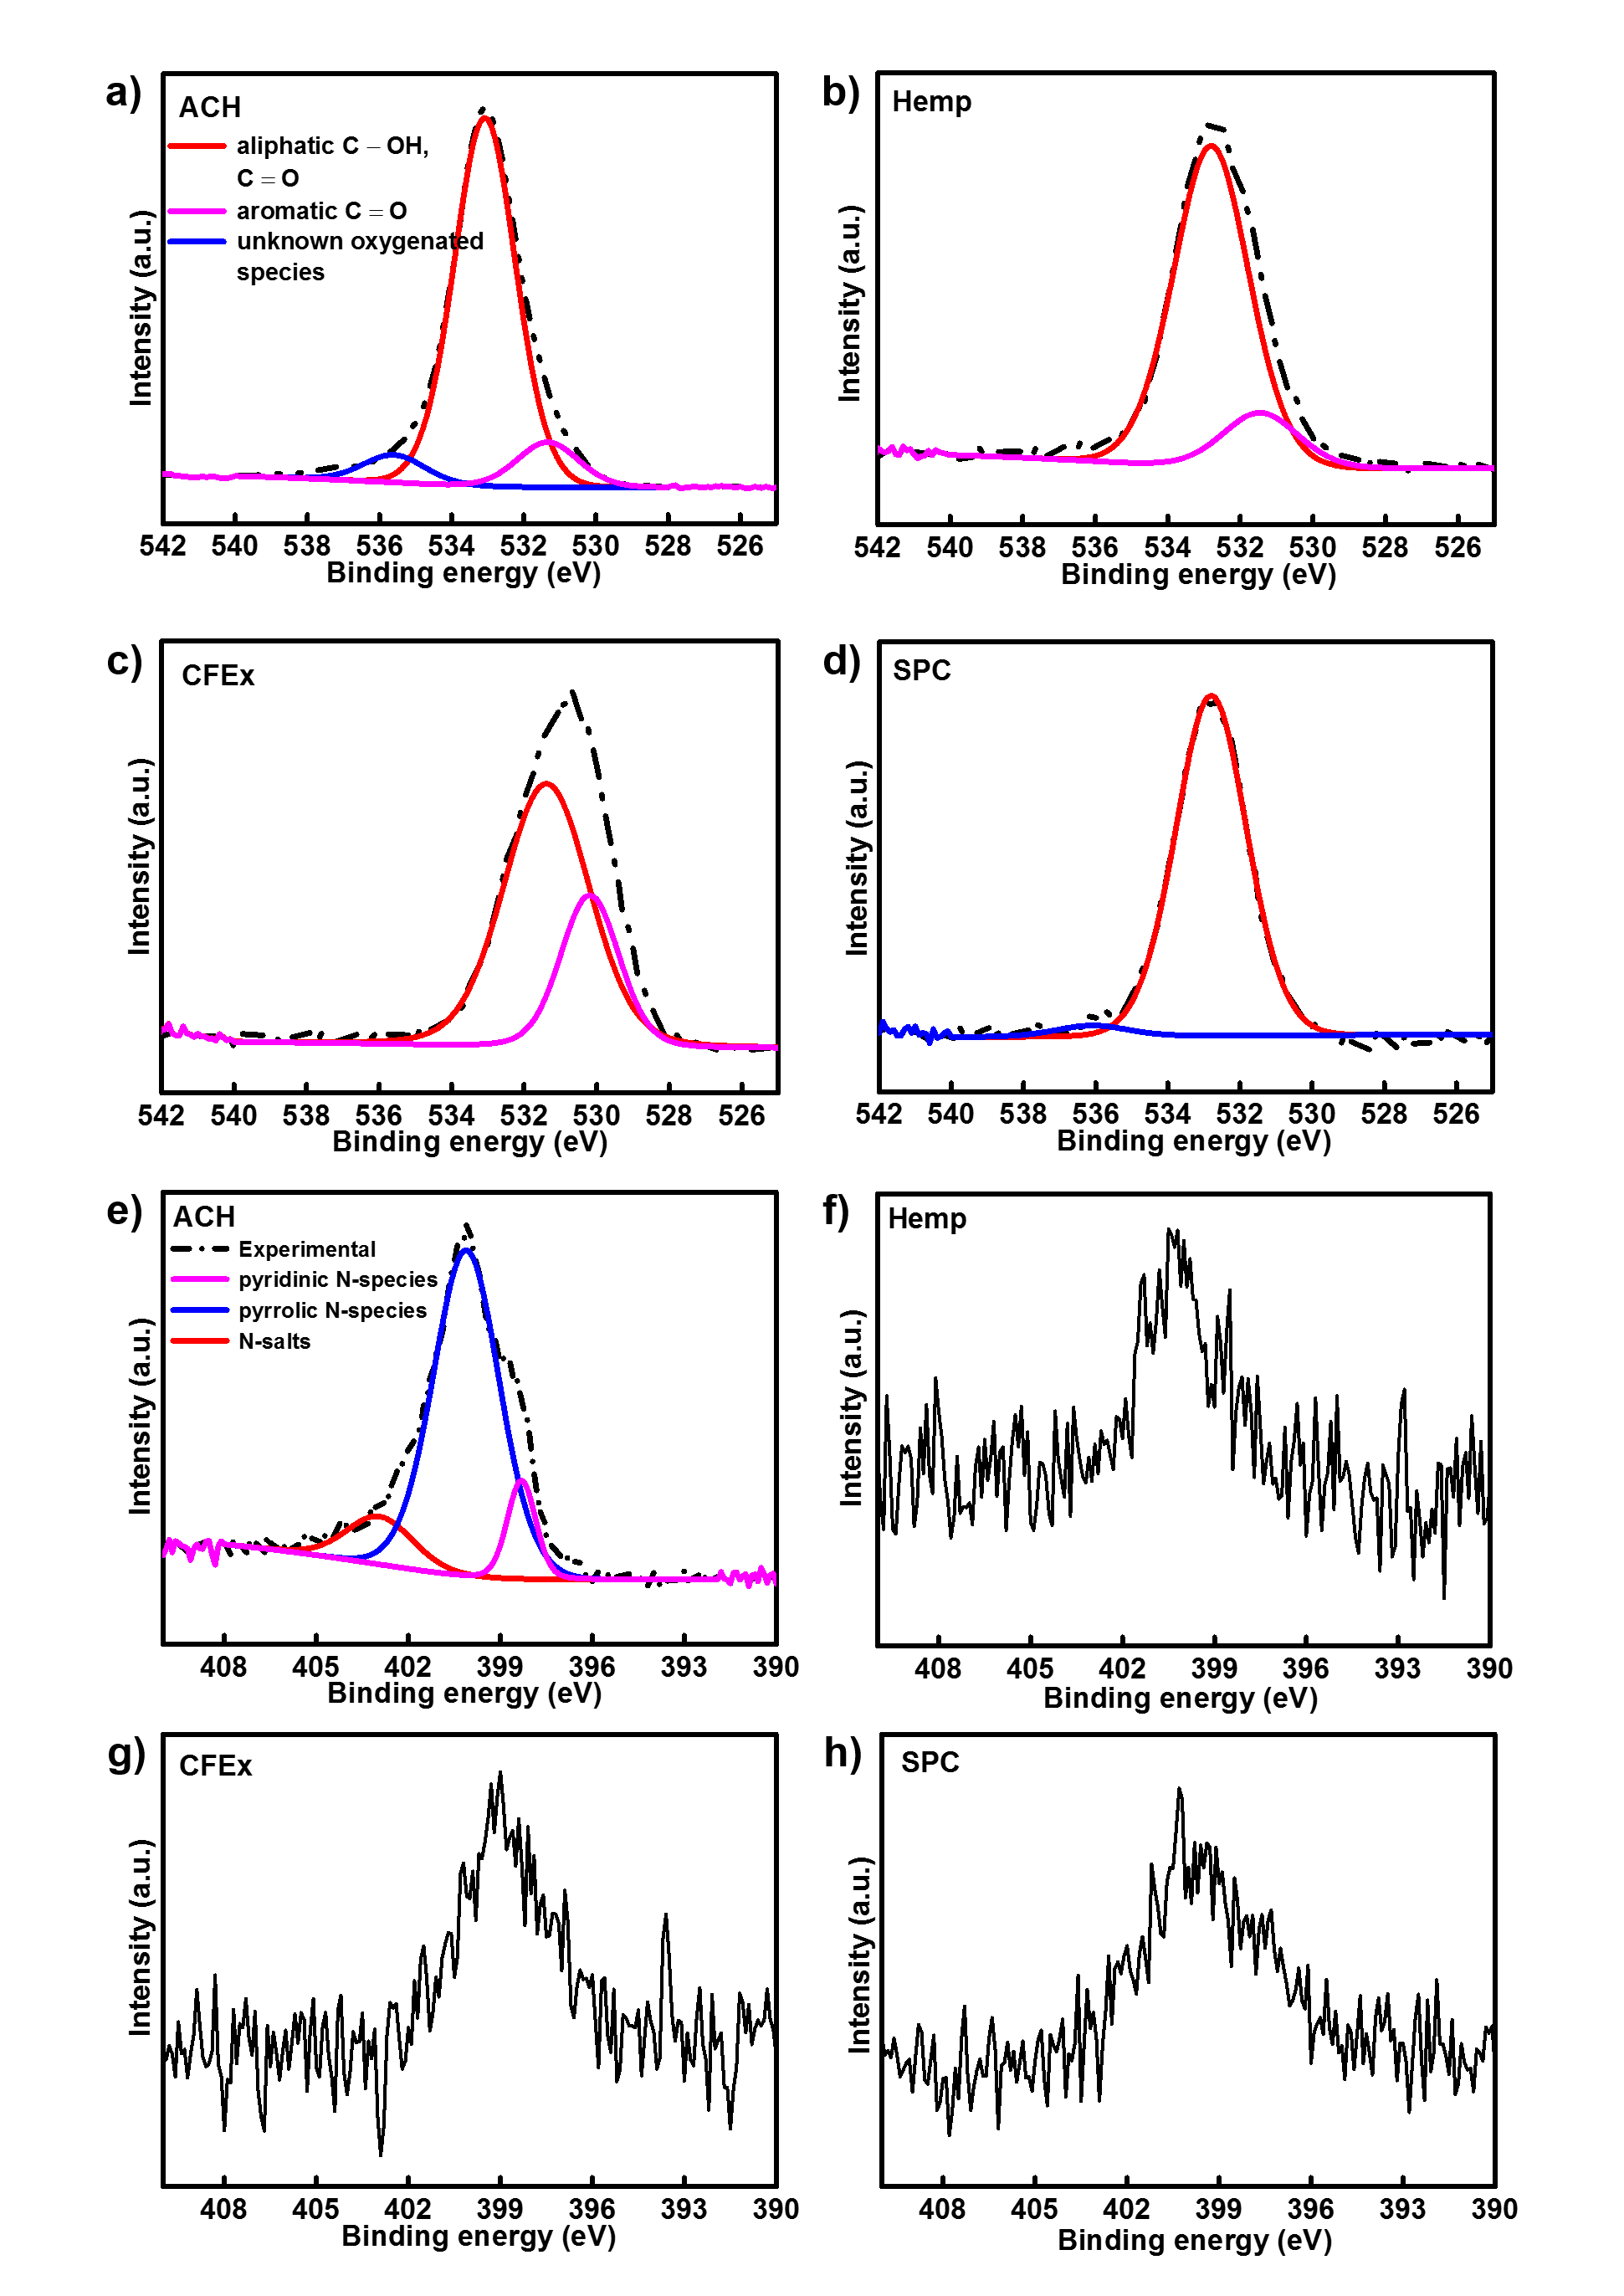
\includegraphics[width=0.8\textwidth]{Figures/chap5fig/xpson}
    \caption{Oxygen 1s orbital XPS spectra of a) ACH, b) hemp fibers c) CFEx and d) Super-P cathodes. ACH and hemp fibers have significant amounts of aliphatic (red) and aromatic (pink) C=O groups present on the cathode surface; while Super-P and CFEx have low amount of oxygenated species at their surface. Nitrogen 1s orbital XPS spectrum of e) ACH, f) hemp fibers g) CFEx and h) Super-P cathodes. ACH displays distinct binding energies for pyridinic and pyrrolic N-species; hemp fibers show lower amount of surface proteins, while Super-P and CFEx have low concentrations of N-containing functional groups.}
  \label{Figures/chap5fig:xpson}
\end{figure}

Figure \ref{Figures/chap5fig:xpson}a-d represents the oxygen 1s peaks of ACH, hemp fibers, CFEx and Super-P cathodes. The peaks at $\approx$ 531 eV stands for an aliphatic -C=O bond. Aromatic C-OH bond has a higher binding energy at $\approx$ 533 eV. The presence of these carbonyl groups not only enhance the wettability of the electrodes, but also suggest towards a Faradaic process\cite{}. 
SPC and CFEx recorded less intense peaks due to negligible amounts C=O and C-O bonds present on their surface. Looking at the nitrogen spectra in Figure , ACH has a distinct presence coming from keratin. Pyrrolic N species have a binding energy at 400.1 eV whereas pyridinic N-species appear at 398.3 eV. Guengen \textit{et al.} suggested that adding nitrogen molecules changed the electron distribution of carbon materials, enhances the wettability of the active material and  contributes to its capacitance \cite{gueguen_xps_2016}. Presence of strong N 1s peaks (Figure \ref{Figures/chap5fig:xpson}e) suggests enhanced wettability of the ACH cathode compared to others, which improves its charge-storage capacity. This might be another reason why ACH cathode recorded a higher specific capacity than other cathodes. 

 \begin{figure}[tbh!]
  \centering
  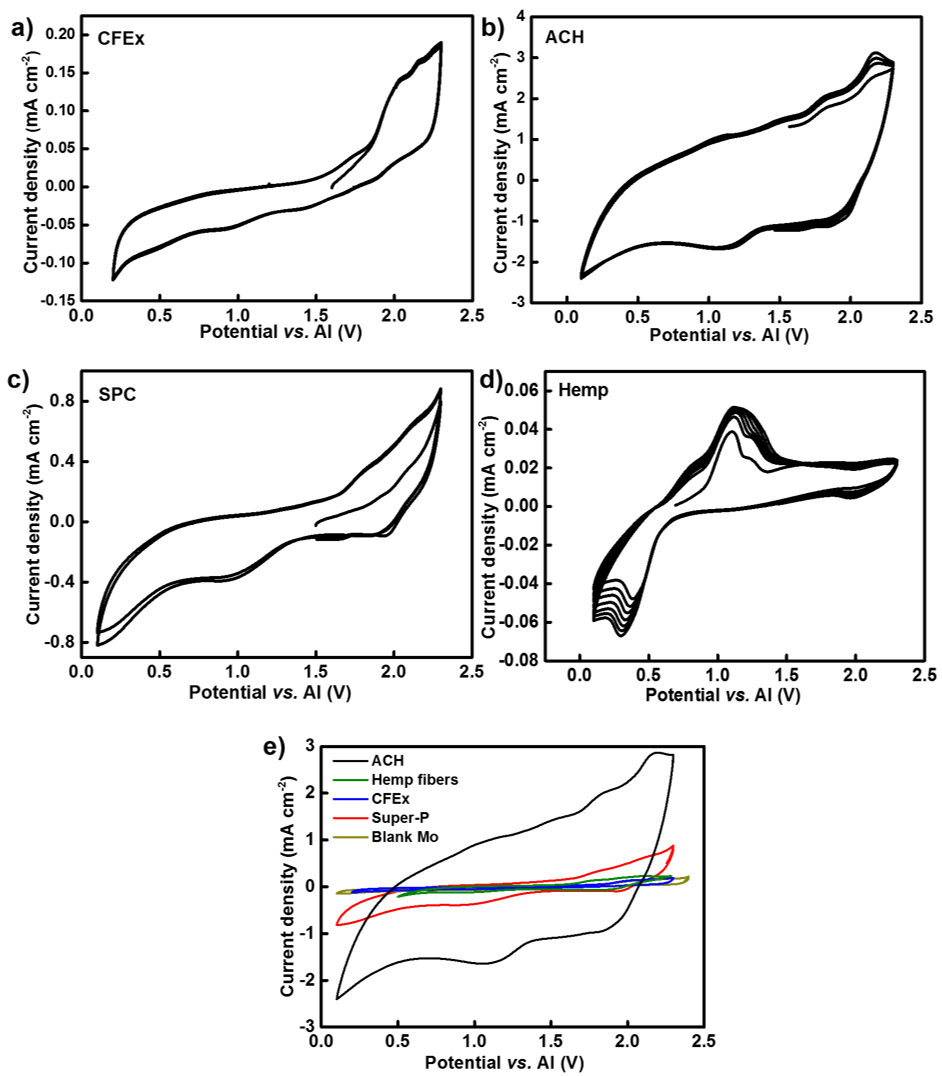
\includegraphics[width=\textwidth]{Figures/chap5fig/CV}
    \caption{Cyclic voltammograms of a) CFEx, b) ACH, c) Super-P and d) hemp fibers cathodes at a scan rate of 10 mV s$^{-1}$ against \ce{Al3+}/Al as a counter/reference electrode in a two-electrode setup. ACH cathode observed a larger CV area than other cathodes, which comes from an additional pseudocapacitance, adding capacity to the system.}
  \label{Figures/chap5fig:CV}
\end{figure}

Lastly, to confirm that ACH is surprisingly a psedocapacitive material, we compared cyclic voltammograms of all the cathodes at a scan rate of 10 mV s$^{-1}$. From Figure \ref{Figures/chap5fig:CV}a-e, it was seen that ACH had a rectangular CV curve. Intercalation process is noticeable at a lower sweep rate (10 mV s$^{-1}$) with tiny redox peaks visible (Figure \ref{Figures/chap5fig:CV}b). Redox pseudo-capacitance, which is usually observed at higher sweep rates (50 mV s$^{-1}$), can be seen in Figure \ref{Figures/chap5fig:hair50mVs}. Since \ce{AlCl4-} anions electrochemically absorb onto the surface of ACH, the  need for long-range diffusion of ions through van der Waals gap decreases. 
ACH proved to be the best carbon-based cathode among all the tested materials, with a specific capacity of 100 mAh g$^{-1}$ at a potential of 1.9 V with a coulombic efficiency of ~90$\%$. Intercalation and deintercalation of \ce{AlCl4-} takes place in the very few graphitic layers of ACH, hemp fibers and Super-P. We found that CFEx lacks a layered structure and it is mainly a cluster of \ce{C60} and \ce{C70} molecules. \ce{AlCl4-} anions seep in and out of the gaps in between the fullerenes changing its structure during insertion and expanding the crystal lattice (Figure \ref{Figures/chap5fig:cfexmech}). Since the cathode maintains its structural integrity, coulombic efficiency remains stable throughout the cycles for CFEx cell. Hemp fibers and Super-P on the other hand, have a highly amorphous structure and degrades after every cycle, resulting in a low capacity value. Figure \ref{Figures/chap5fig:cfexachlong} compares the 50th cycle measurement for Al/ACH and Al/natural graphite cell. It not only displays a higher specific capacity than conventional graphite, but also a high battery voltage of 1.92 V with an energy density of 202 Wh kg$^{-1}$.

 \begin{figure}[tbh!]
  \centering
  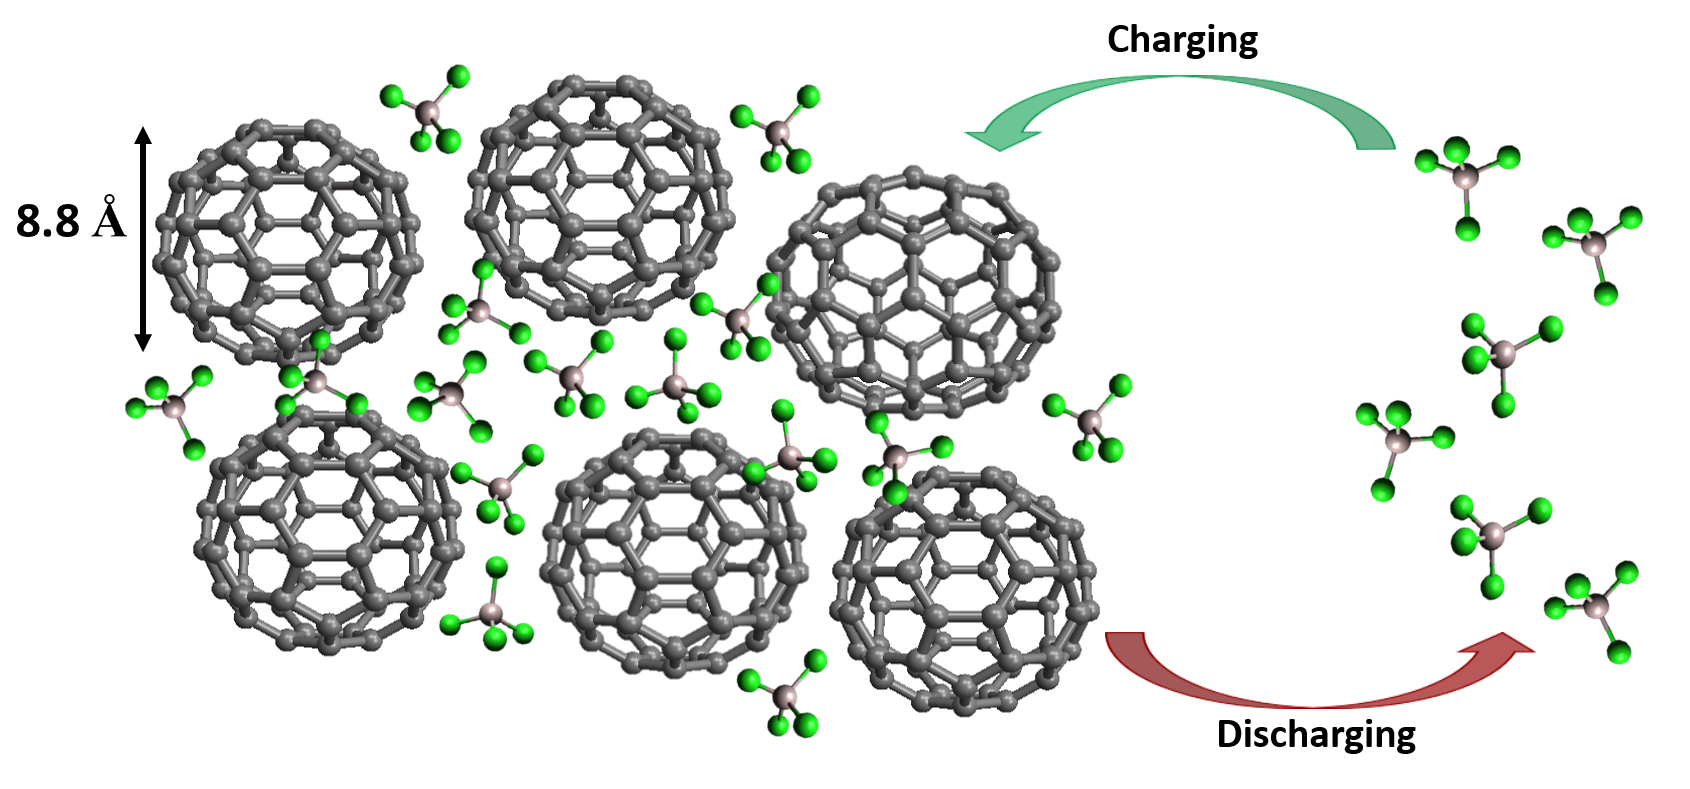
\includegraphics[width=\textwidth]{Figures/chap5fig/cfexmech}
    \caption{Suggested mechanism for a \textbf{Al/CFEx} cell. \ce{AlCl4-} ions seeping in through the gaps present between fullerene molecules. A few \ce{AlCl4-} ions get absorbed on the cathode's surface resulting in a capacity purely from a non-Faradaic process.}
  \label{Figures/chap5fig:cfexmech}
\end{figure}

\begin{figure}[tbh!]
  \centering
  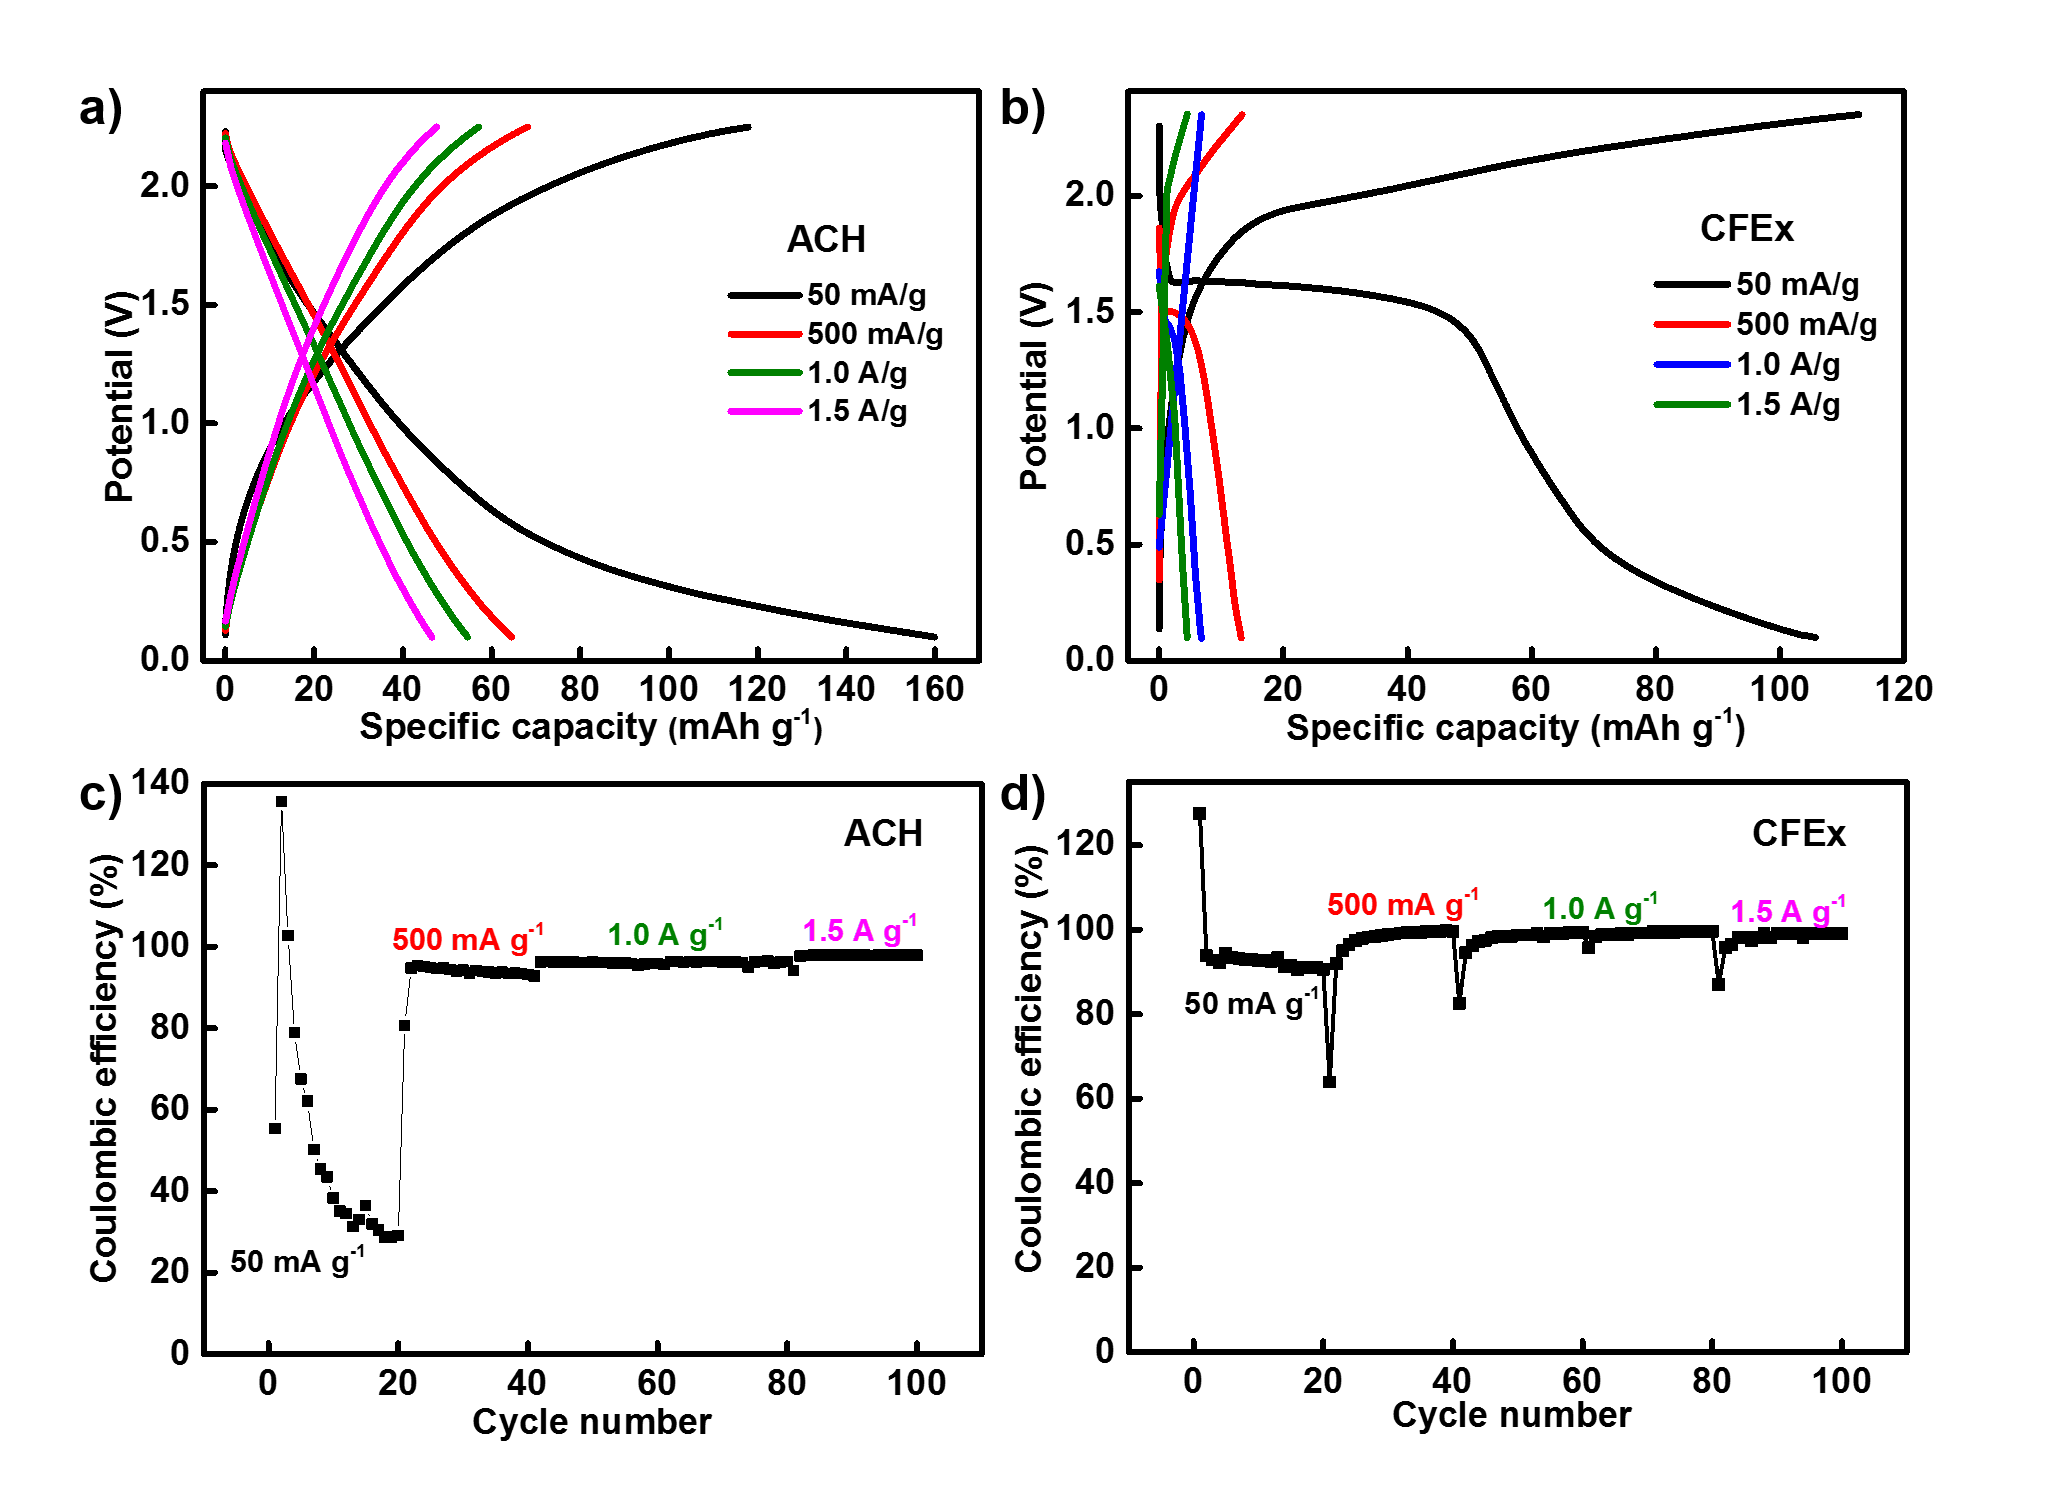
\includegraphics[width=\textwidth]{Figures/chap5fig/cfexachlong}
    \caption{Discharge capacities of a) ACH and b) CFEx cathodes at current rates of 50mAg$^{-1}$, 500mAg$^{-1}$, 1.0 Ag$^{-1}$ and 1.5 Ag$^{-1}$ along with their coulombic efficiencies. }
  \label{Figures/chap5fig:cfexachlong}
\end{figure}

\section{Experimental methods}

\subsection{Cathode preparation}
Slurry was prepared by mixing the active material (85$\%$ by wt.), 9$\%$ binder (PVDF, MTI Corp.) and 6$\%$ Super-P conductive carbon (99+$\%$ metals basis, Alfa Aesar) in N-methyl pyrrolidone NMP (anhydrous, 99.5$\%$, Sigma-Aldrich). For SPC slurry 94$\%$ active material and 6$\%$ binder was mixed together to form a slurry. It was ‘doctor-bladed’ on molybdenum foil used as a conductive substrate (thickness 0.1 mm, MTI Corp.) and dried in a vacuum oven at 120$^{\circ}$C for 12 hours to adhere the slurry on the substrate and evaporate the solvent. Specific loading of the materials ranged from 11-12 mg cm$^{-2}$.

\subsection{Electrolyte preparation}
Anhydrous \ce{AlCl3} (Sigma-Aldrich) and EMImCl (97$\%$, Sigma-Aldrich) were mixed in a molar ratio of 1.3:1, at room temperature. EMImCl was baked in vacuum for 24 hours at 100$^{\circ}$C to remove residual moisture. Small aliquots of \ce{AlCl3} was added to EMImCl after every few minutes. The ionic liquid was stirred for 2-3 hours until a clear brown liquid was obtained. Since the electrolyte is hygroscopic in nature, it was prepared in a \ce{N2}-filled glove box with <0.1 ppm \ce{H2O}/\ce{O2}. 

\subsection{Cell assembly}
PEEK (polyether ether ketone) cells were used for electrochemical measurements. Molybdenum rods were used as current collectors. It was seen previously that steel rods reacted with the electrolyte forming a green-colored substance on the cathode. Slurry coated on molybdenum foil was used as the cathode and placed at bottom of the cell. Two glass microfibers (Grade GF/F, Whatman) were used as separators. 80$\mu$l of the electrolyte was used to wet the separator. Aluminium foil (thickness 0.1 mm, 99$\%$, GoodFellow) used as an anode and placed on top of the separator. It was assembled in a \ce{N2}-filled glove box. The cell was then sealed and wrapped with a paraffin film to avoid any air or moisture contact. Since this was a two-electrode setup, aluminium foil was used as both counter and reference electrode. The cell was taken out of the glove box and electrochemical measurements were performed. 

\begin{figure}[tbh!]
  \centering
  
\includegraphics[width=\textwidth]{Figures/chap5fig/gcdall}
    \caption{Chronopotentiographs (Voltage vs. Time) curves of all tested cathodes.}
  \label{Figures/chap5fig:gcdall}
\end{figure}

\begin{figure}[tbh!]
  \centering
  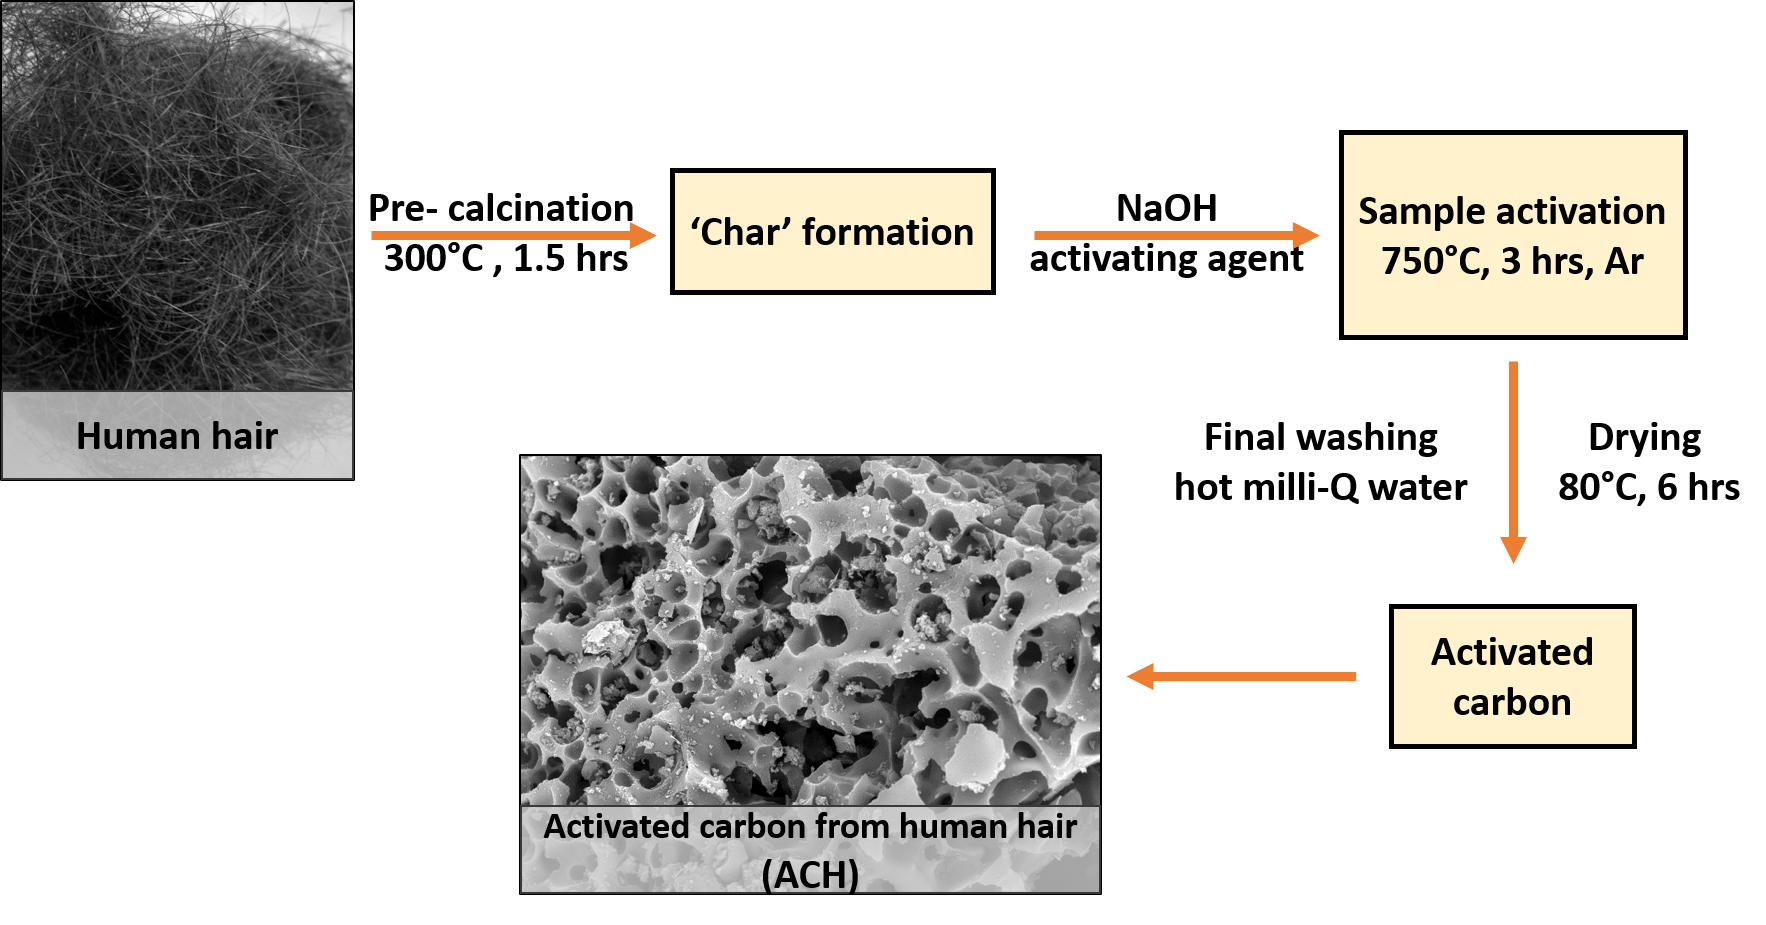
\includegraphics[width=\textwidth]{Figures/chap5fig/achsyn}
    \caption{Synthesis of activated carbon from human hair using NaOH as the activating agent. The choice of temperature and activating agent plays a crucial role in determining pore size of the activated carbon.}
  \label{Figures/chap5fig:achsyn}
\end{figure}

\begin{figure}[tbh!]
  \centering
  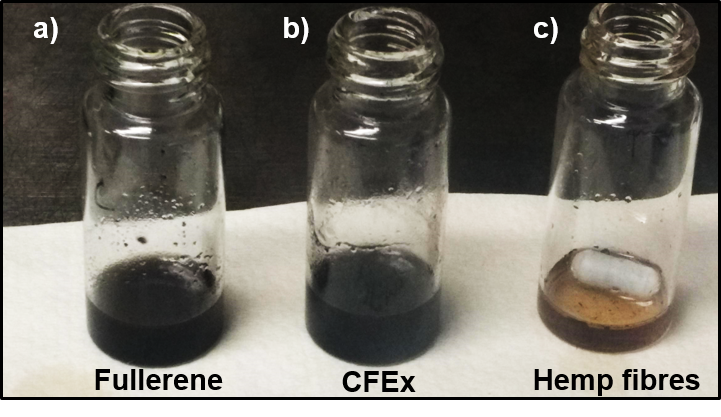
\includegraphics[width=\textwidth]{Figures/chap5fig/cfexsol}
    \caption{Synthesis of activated carbon from human hair using NaOH as the activating agent. The choice of temperature and activating agent plays a crucial role in determining pore size of the activated carbon.}
  \label{Figures/chap5fig:cfexsol}
\end{figure}

\begin{figure}[tbh!]
  \centering
  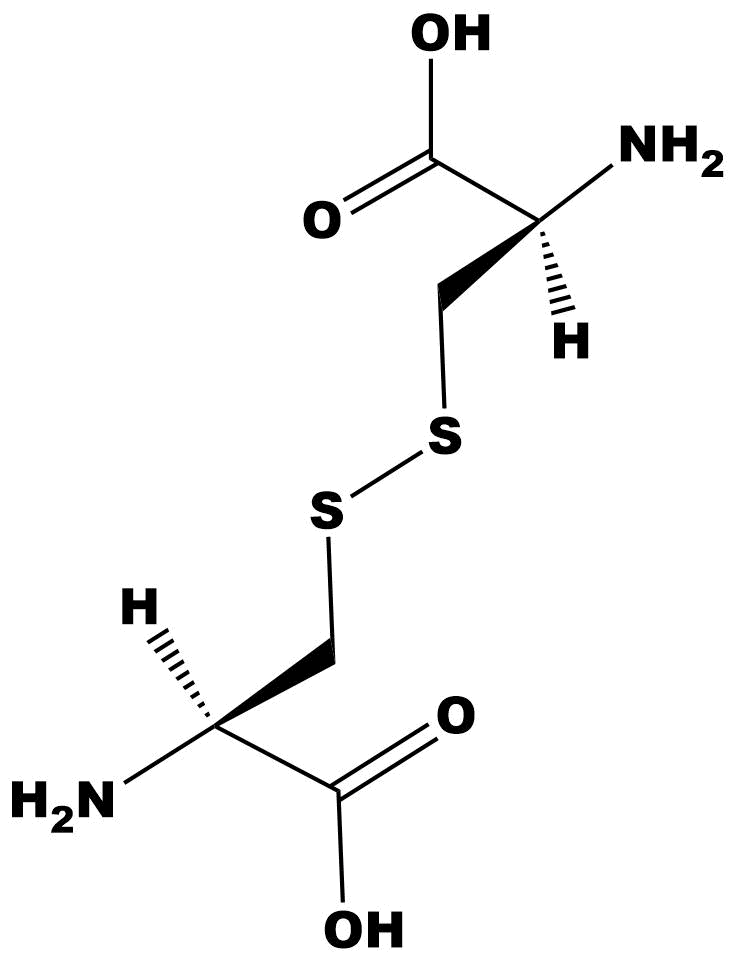
\includegraphics[width=0.5\textwidth]{Figures/chap5fig/keratin}
    \caption{Keratin: a protein abundantly found in human hair contains C-O, C=O, C-NH$_2$ bonds.} 
    \label{Figures/chap5fig:keratin}
\end{figure}

\begin{figure}[tbh!]
  \centering
  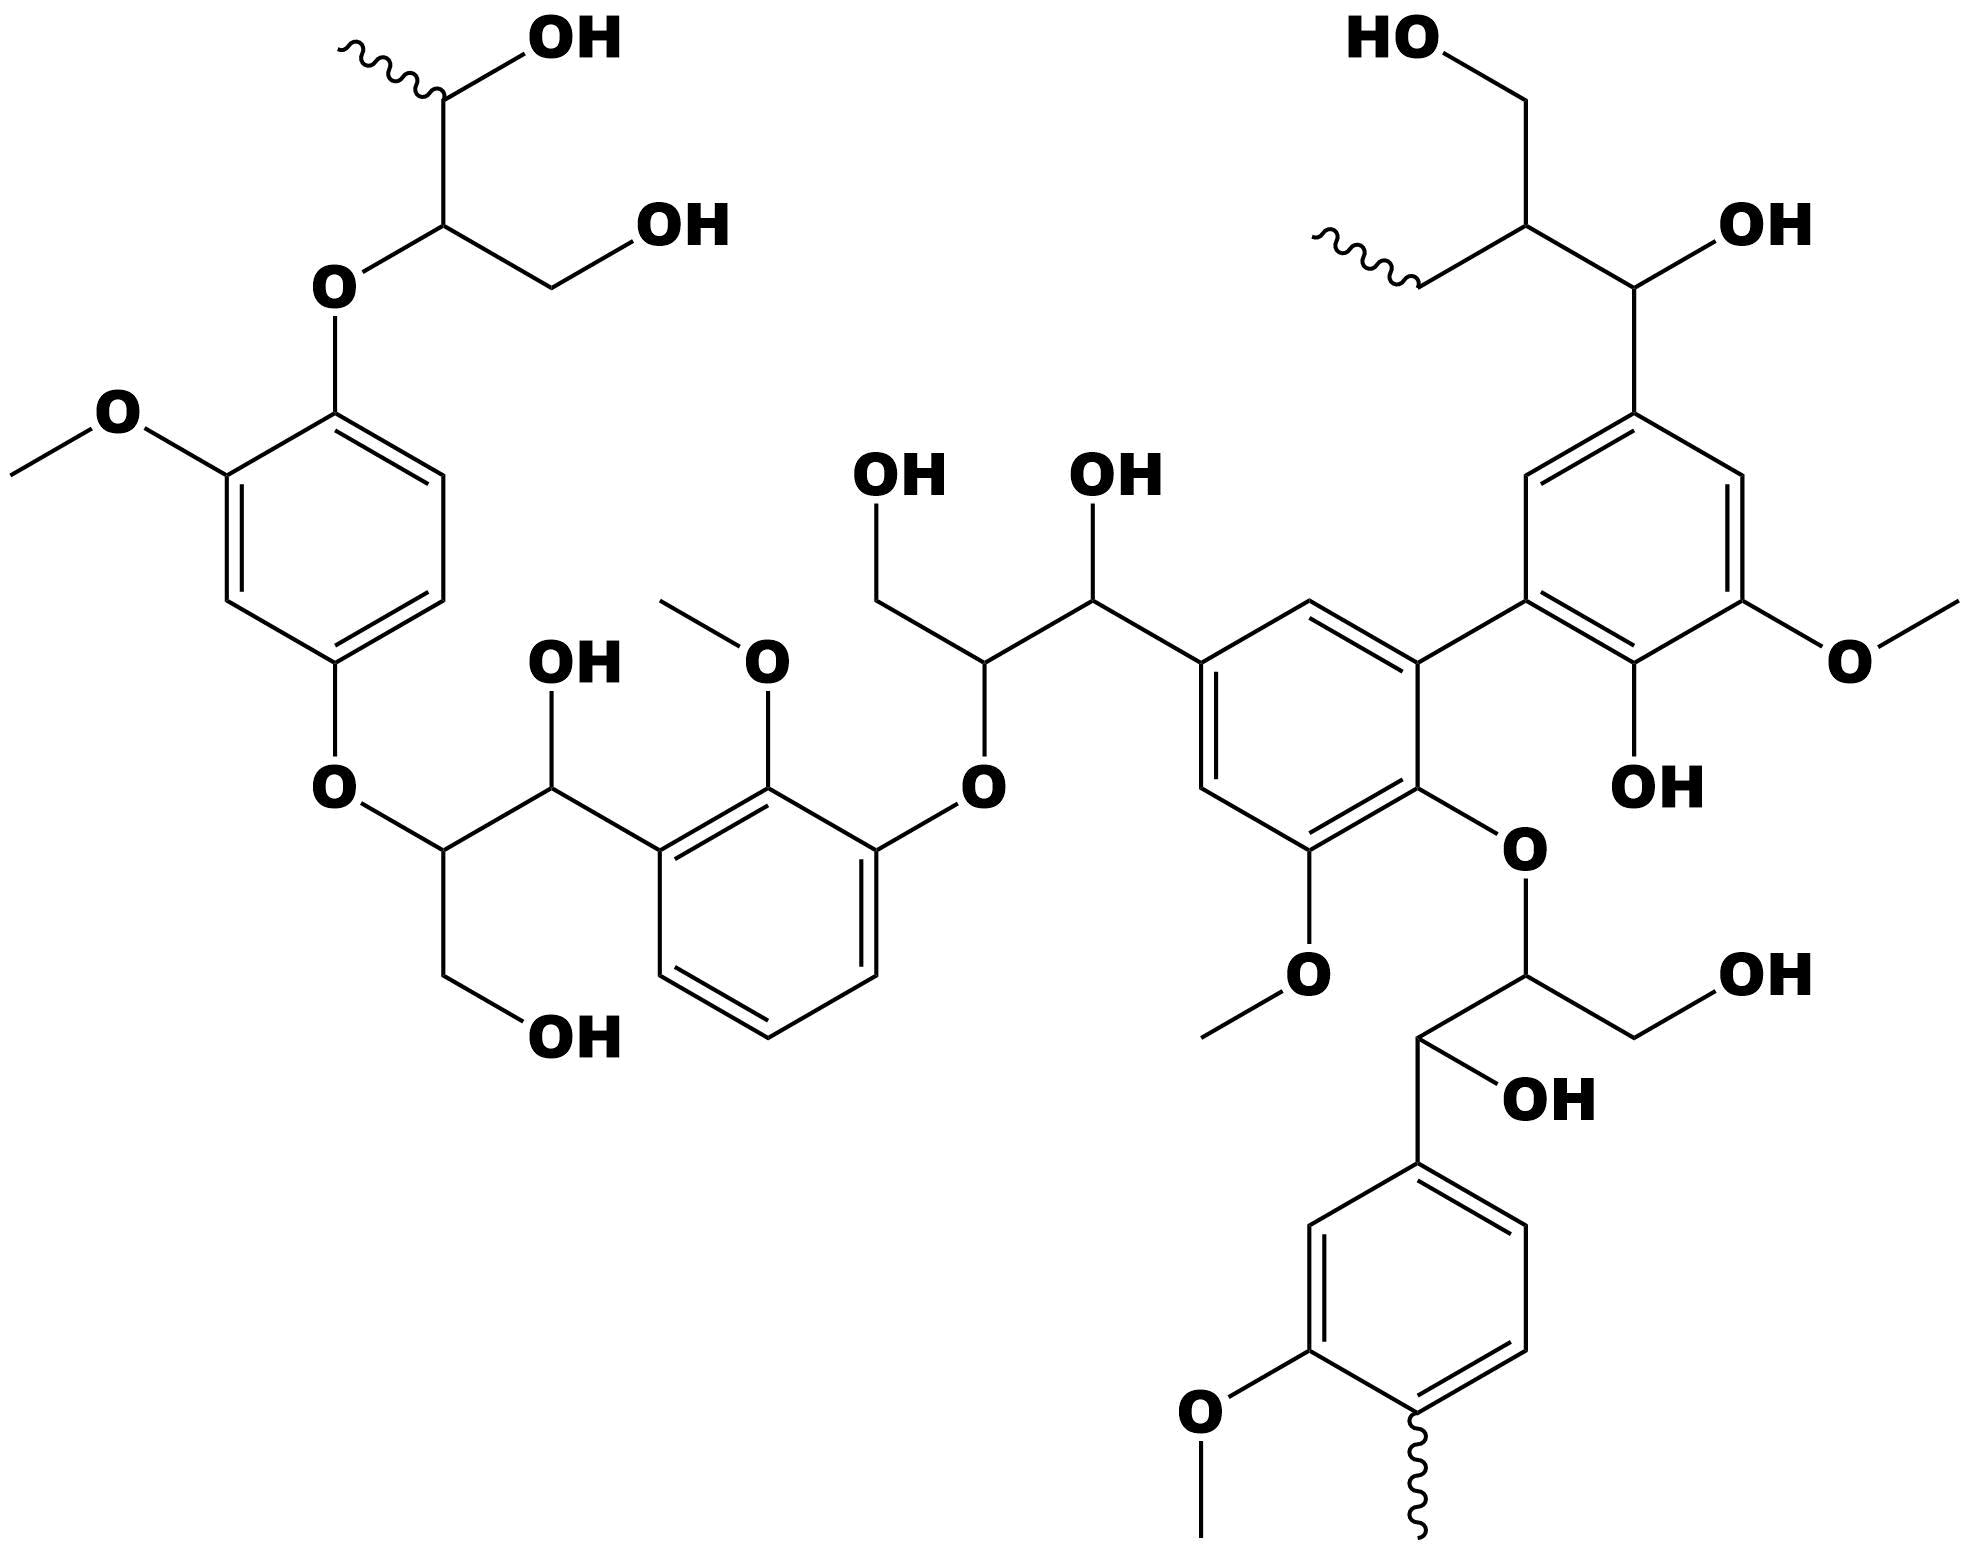
\includegraphics[width=0.5\textwidth]{Figures/chap5fig/lignin}
    \caption{Structure of Lignin- The lignin content of hemp will vary according to the part of the plant under observation. It contains a number of carbonyl, ester groups along with other proteins such as edestin and albumin.}
  \label{Figures/chap5fig:lignin}
\end{figure}

\begin{figure}[tbh!]
  \centering
  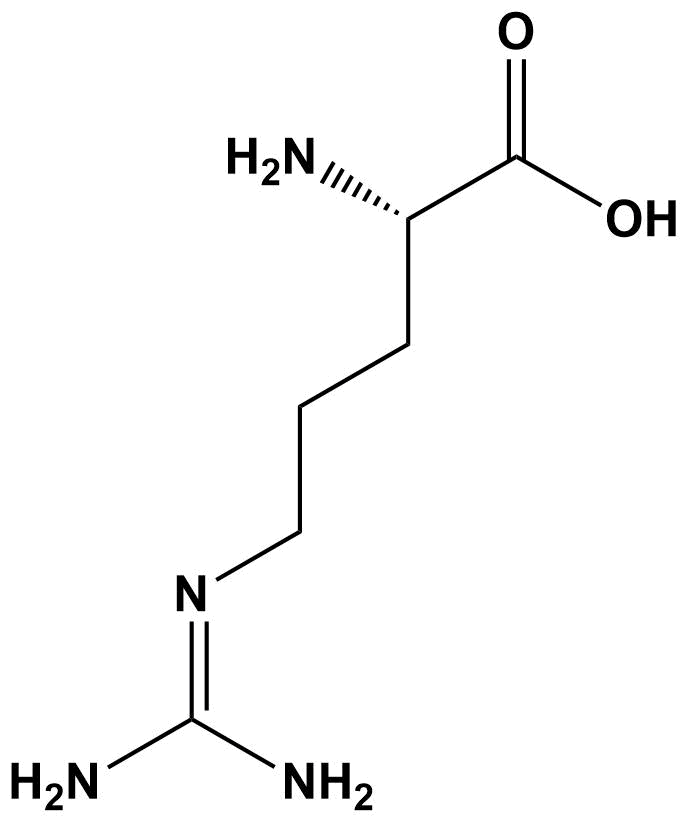
\includegraphics[width=0.5\textwidth]{Figures/chap5fig/arginine}    
  \caption{Structure of Arginine- major component of hemp fibers containing C-N, C=O, C-O bonds.}
  \label{Figures/chap5fig:arginine}
\end{figure}

\begin{figure}[tbh!]
  \centering
  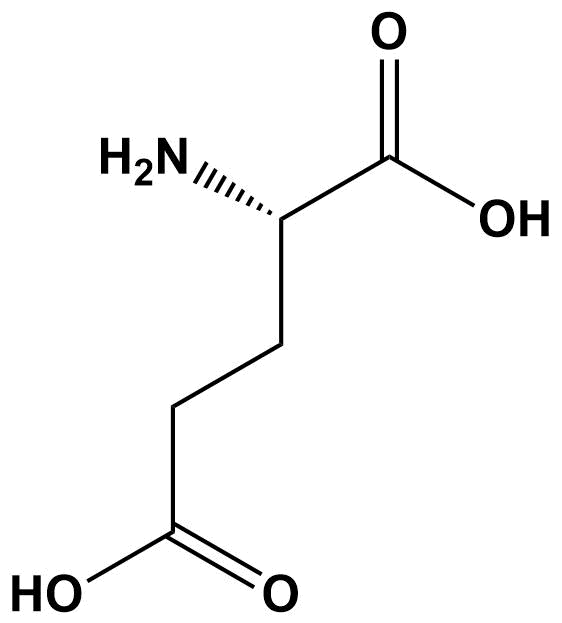
\includegraphics[width=0.5\textwidth]{Figures/chap5fig/gluacid}
    \caption{Structure of Glutamic acid- another protein found in hemp fibers containing C-O, C=O and C-N bonds.}
  \label{Figures/chap5fig:gluacid}
\end{figure}

\begin{figure}[tbh!]
  \centering
  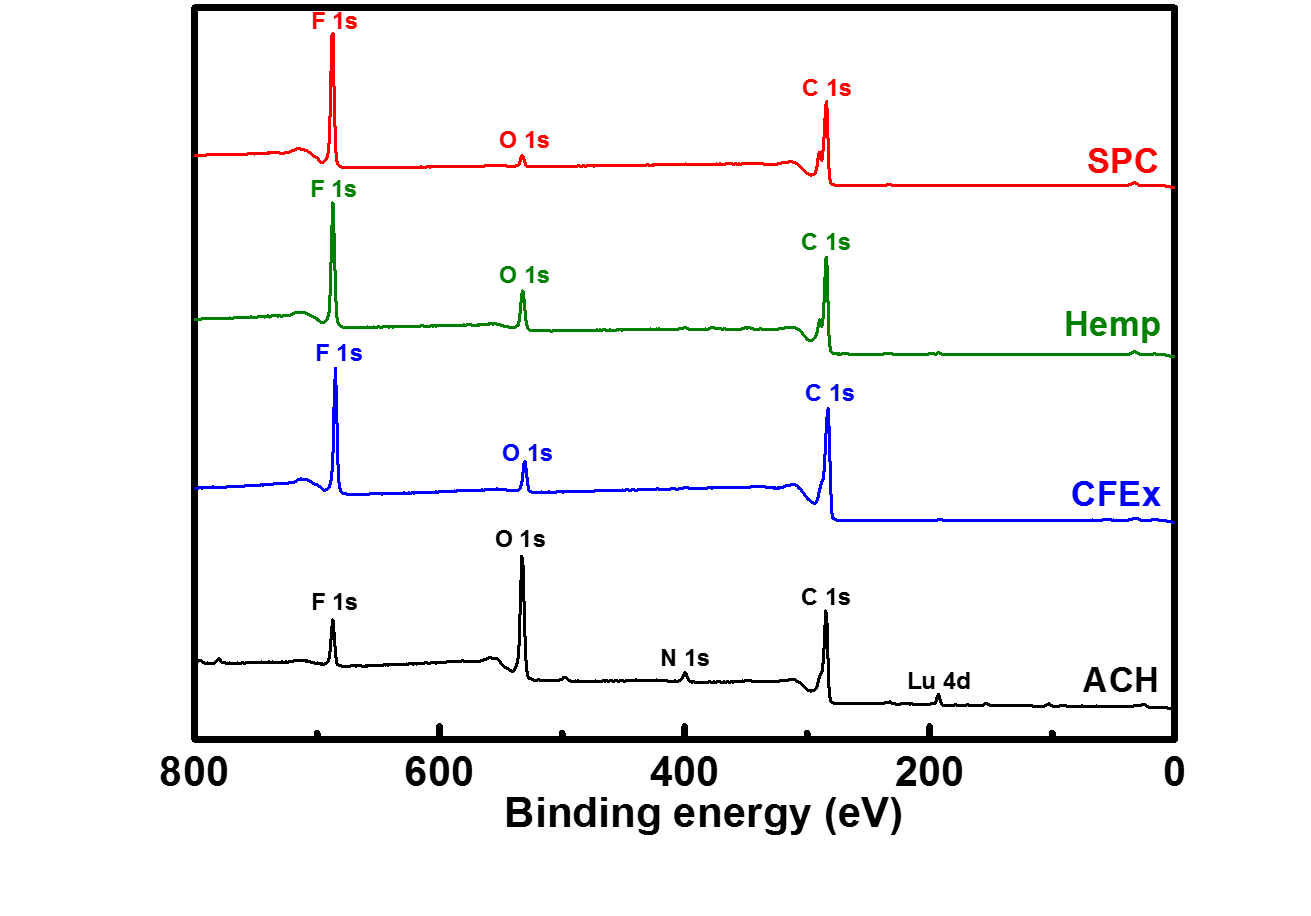
\includegraphics[width=\textwidth]{Figures/chap5fig/xpsoverall}
    \caption{Overall spectra of ACH (blck), hemp fibers (blue), CFEx (green) and SUper-P(red).}
  \label{Figures/chap5fig:xpsoverall}
\end{figure}

\begin{figure}[tbh!]
  \centering
  
\includegraphics[width=\textwidth]{Figures/chap5fig/hair50mVs}
    \caption{Cyclic voltammogram of ACH at a scan rate of 50 mV/s in a two electrode setup against \ce{Al3+}/Al showing a capacitor-like behaviour with no visible oxidation-reduction peaks unlike Figure \ref{Figures/chap5fig:CV}b where we distinctly observed redox peaks.}
  \label{Figures/chap5fig:hair50mVs}
\end{figure}

\section{Conclusion and future outlook}

